\chapter{Coatings for CAST}
After the launch of NuSTAR, the X-ray optics group at DTU Space was invited to participate in the creation of an X-ray optic for the CAST solar axion helioscope \cite{Elias:1387488,Iguaz:1389411}. CAST is an experiment at CERN that looks for the hypothetical axion particle\cite{Weinberg:1978ii,Wilczek:1978kp,Peccei:1977ea,Peccei:1977em} which is a solution to the charge-parity (CP) problem of the standard model in particle physics\cite{Cheng:1988fu}. If the axion exist, it constitutes some or all of the Dark Matter in the universe\cite{Visinelli:2011tw,Bae:2008ix}. It was decided that the optics technology from NuSTAR\cite{Christensen:2011wg,Harrison:2010gu,Koglin:2005kb,Zhang:2009cb,Harrison:2013wl} could be leveraged and therefore use spare glass to make an inexpensive and relatively simple X-ray optic.

The optic was designed between summer 2012 and summer 2014. Production, assembly, installation and alignment with CAST was done during summer 2014 in cooperation with University of Zaragoza (UoZ) in Spain and Lawrence Livermore National Lab (LLNL) in the US. In this chapter the reader will find a description of the whole process from start to finish.

My part of the work was to design the optic geometry and coating as well as produce the coated substrates and participate in the installation. LLNL designed the vacuum vessel and alignment procedure and UoZ designed detector and the X-ray source assembly.

A complete software package was developed that could calculate the geometry of the optic given a focal length and substrate specifications. The software then optimises the coating for a range of material combinations with respect to energy range and axion spectrum by incorporating IMD. I chose to make the software in Python because of the huge amount of documentation and specialised packages available. To interface with IMD, a package called Pidly was used to communicate with IDL, which could spawn an IMD session. The principle is described in section \ref{sec:software_improvements}

\section{The CAST instrument}
The axion is an ultra-light particle that is formed from the interaction of a photon with an electromagnetic field, called the Primakoff effect. A primary source of the particle would be from inside stars, and from Earth the best nearby source will of course be the Sun. The axion is weakly interacting so in order to detect it, CAST uses a strong magnet to convert the axion back to a photon, again by the Primakoff effect. The photons subsequently hit a detector.

\begin{figure}[htbp]
  \centering
    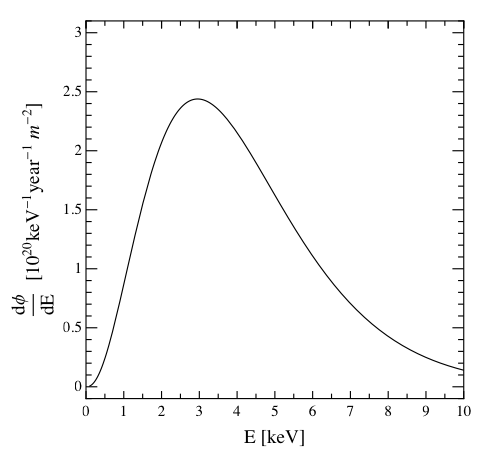
\includegraphics[height=6cm]{figures/cast/axion_spectrum.png}
  \caption{\footnotesize Solar axion flux spectrum at Earth. }
  \label{fig:axion_spectrum}
\end{figure}

The spectrum of X-rays from solar axions reaching Earth can be seen in figure \ref{fig:axion_spectrum}. It is relatively low energy X-rays with a peak around 3 keV and a shape similar to the black-body radiation spectrum.

\begin{figure}[htbp]
  \centering
    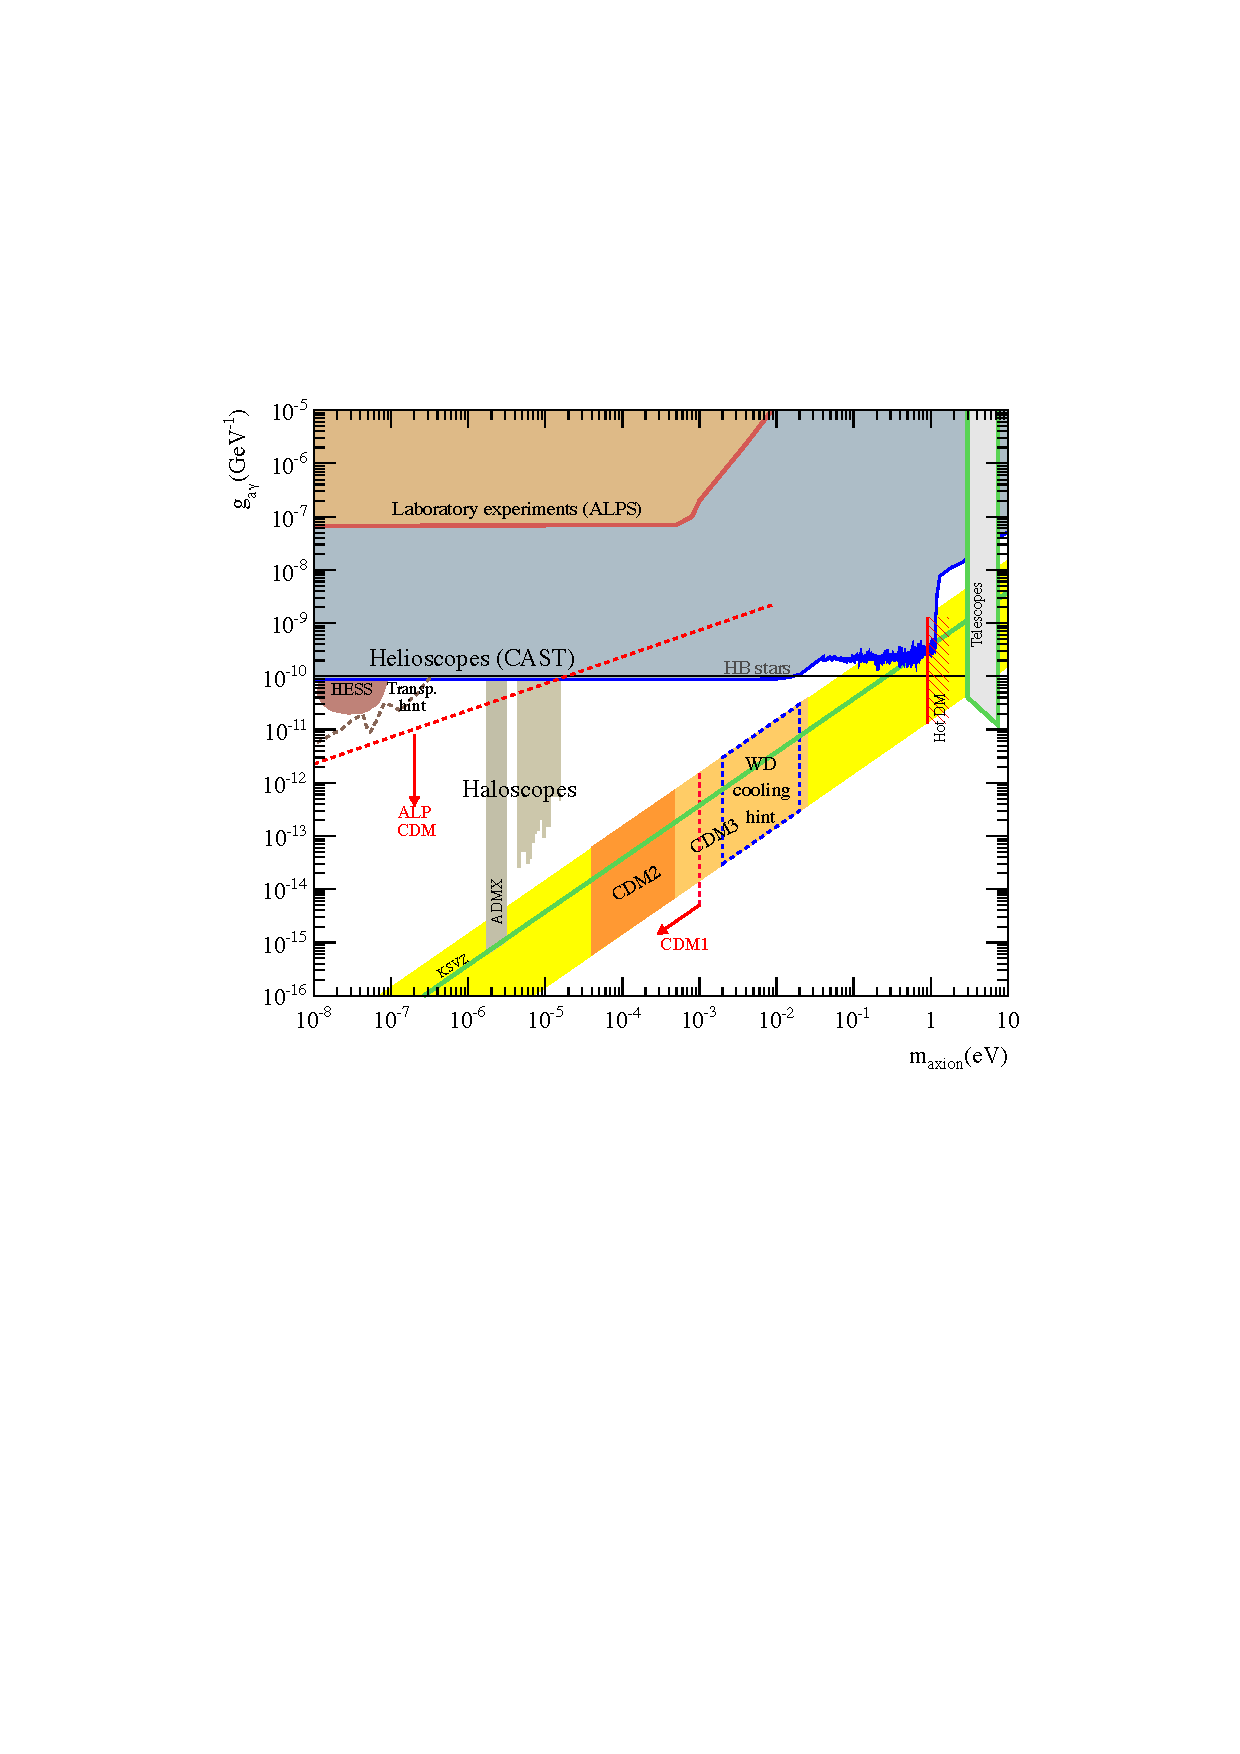
\includegraphics[height=6cm]{figures/cast/axion_search_cast2.pdf}
  \caption{\footnotesize The axion (and axion-like partikle) parameter space, showing the limits of detection for current direct detection experiments. The yellow "axion band" represents areas of the parameter space where theoretical models predicts axions. The part of the parameter space excluded by the CAST axion helioscope so far is represented by the blue line and grey area. (From \cite{Irastorza:2013uu})}
  \label{fig:axion_search_cast}
\end{figure}

Cosmological observations constrain the axion mass between 1 $\upmu$eV and 1 eV. In figure \ref{fig:axion_search_cast} the parameter space can be seen with the axion-photon coupling constant, \gay, as a function of the axion mass, \maxion. The yellow line represents the area where we expect to see the axion if all dark matter in the universe consists of axion particles with the same \maxion\ and \gay. The CAST helioscope is by 2014 the most comprehensive axion search, and has set an experimental upper limit of
\begin{eqnarray}
\gaymath \leq 8.8 \cdot 10^{-11} \textrm{ GeV}^{-1}\cite{Zioutas:2005jl,Andriamonje:2007jc}.
\end{eqnarray}
% \begin{figure}
% \centering
% \begin{minipage}{.5\textwidth}
%   \centering
%   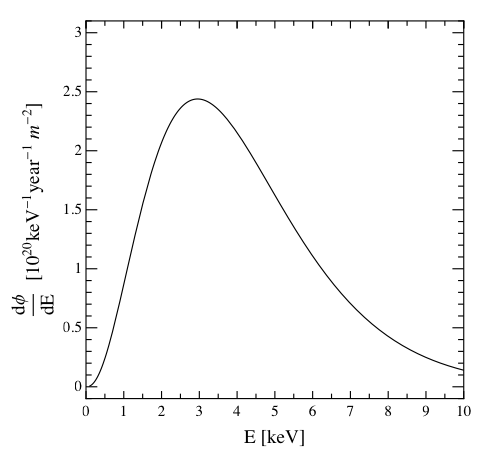
\includegraphics[height=4.6cm]{figures/cast/axion_spectrum.png}
%   \captionof{figure}{A figure}
%   \label{fig:axion_spectrum}
% \end{minipage}%
% \begin{minipage}{.5\textwidth}
%   \centering  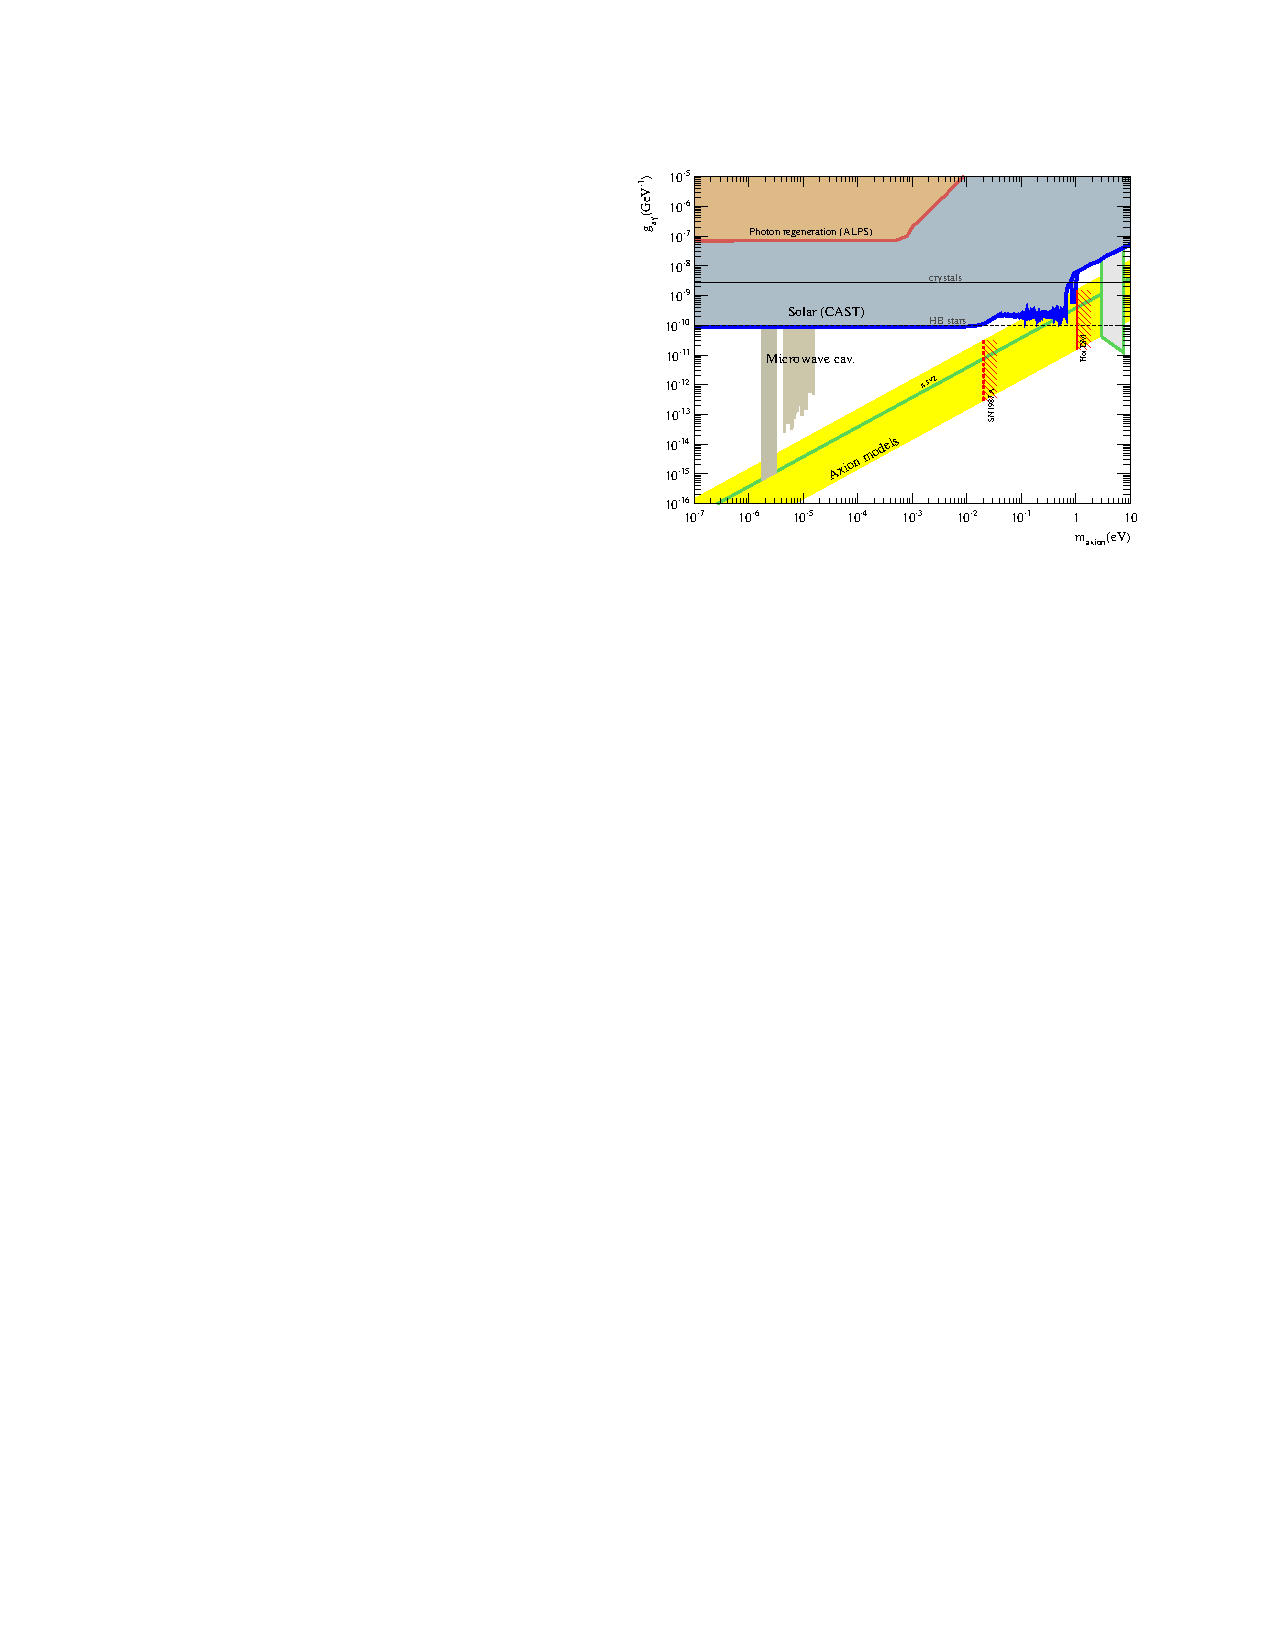
\includegraphics[width=\linewidth]{figures/cast/axion_search_cast.pdf}
%   \captionof{figure}{Another figure}
%   \label{fig:axion_search_cast}
% \end{minipage}
% \end{figure}
The CAST experiment is largely made from spare parts of other projects at CERN and other research institutions. The magnet is one of three prototype superconducting dipole magnets from the Large Hadron Collider. It is designed to transport particles in two directions inside a strong magnetic field, so it has two bores inside with diameters of 43 mm. As can be seen in the picture of the CAST instrument (figure \ref{fig:cast_instrument}), the magnet is able to pitch and yaw up to a limit. That makes it possible to follow the sun as it comes up with one end, and as it goes down with the other end. Since the axion does not interact with matter, detectors are placed at both ends of the magnet and at both boreholes, so two detectors can be used at sunrise and two at sunset. The detectors used are low-background time projection chambers with MicroMegas readouts \cite{Giomataris:1996eo,Giomataris:2006fy,Andriamonje:2010jh}.

\begin{figure}[htbp]
  \centering
    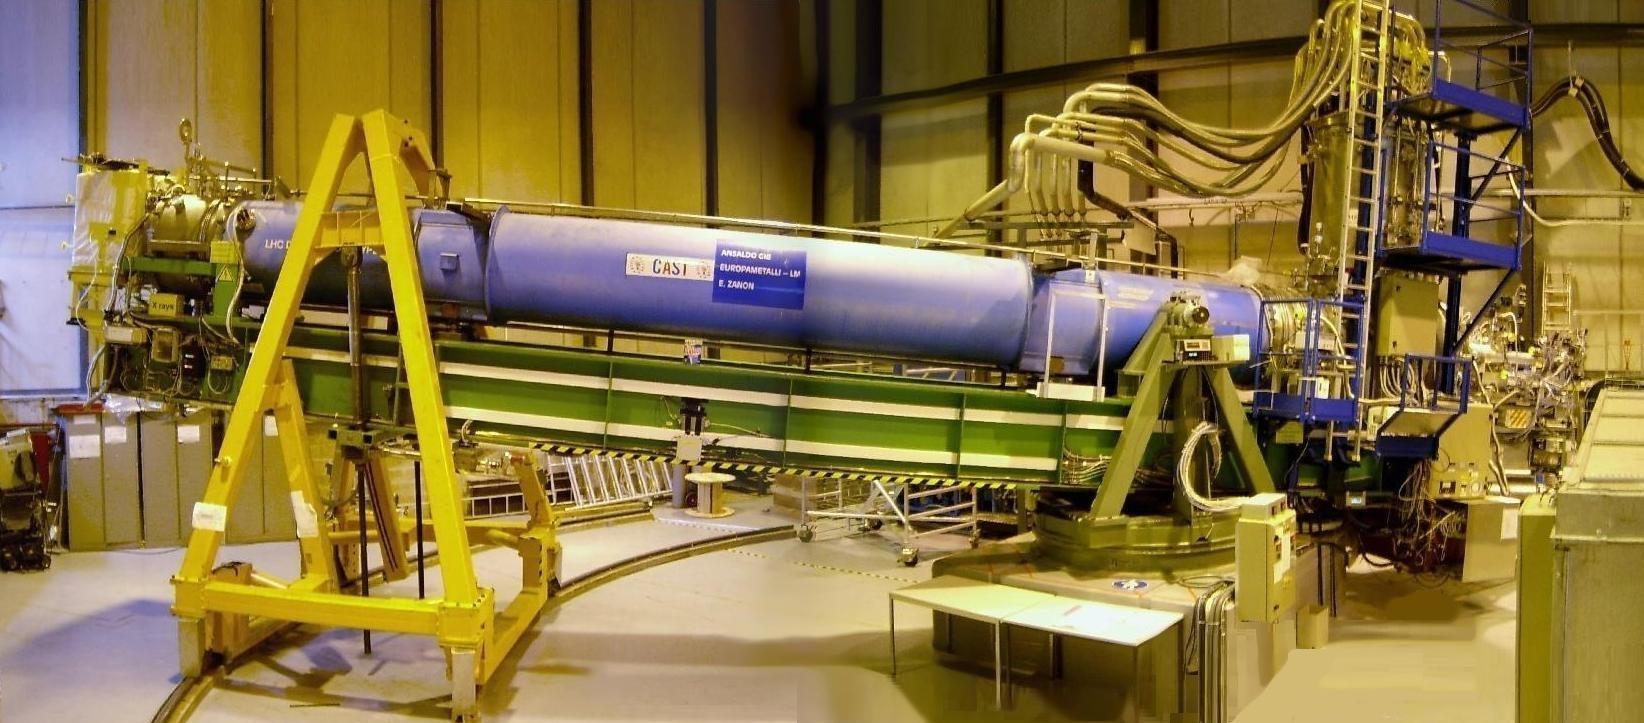
\includegraphics[height=5cm]{figures/cast/cast_instrument.jpg}
  \caption{\footnotesize The Cern Axion Solar Telescope (CAST) located near Geneva, Switzerland. The main component of the experiment is a Large Hadron Collider (LHC) prototype dipole magnet that has a 10 T magnetic field, physical length of 13 meters and a mass of 50 tonnes.}
  \label{fig:cast_instrument}
\end{figure}

CAST has been doing axion searches since 2002 and the experiment continually improves and reiterates the equipment to get higher sensitivity. One major problem is to get a high enough signal-to-noise ratio, the majority of the noise coming from background radiation from the ground, the materials in the instrument and cosmic rays. The detectors cover the entire area of each bore opening, so are relatively large. Detector size is proportional to the background radiation, so it makes sense to have smaller detectors. By using X-ray optics, the X-ray photons can be focused into a detector area of only a fraction of the previous. This will significantly increase the signal-to-noise ratio and will let the CAST helioscope search for the axion in new areas.

\section{Developing an optic for CAST}
One major concern in making an X-ray optic from NuSTAR glass for the CAST helioscope is the limited space available. The optic would have to fit on the end of the magnet nearest the wall, which leaves only about 2 meters for optic, detector and the focal length between the two. Another problem is the small bore opening of only 43 mm, which is smaller than the inner radius of the NuSTAR telescopes. Both of those problems can be solved by realising that the optic does not require a symmetric field of view and that the axion spectrum is of relatively low energies. In figure \ref{fig:cast_xrt_principle} is seen a top-down view of the end of the magnet bore where the optic and detector can be attached. By stacking a number of reflectors, X-rays can be reflected to one side, something that would not be possible for a traditional imaging X-ray astrophysical telescope.

\begin{figure}[htbp]
\centering
\begin{minipage}{.40\textwidth}
  \centering
  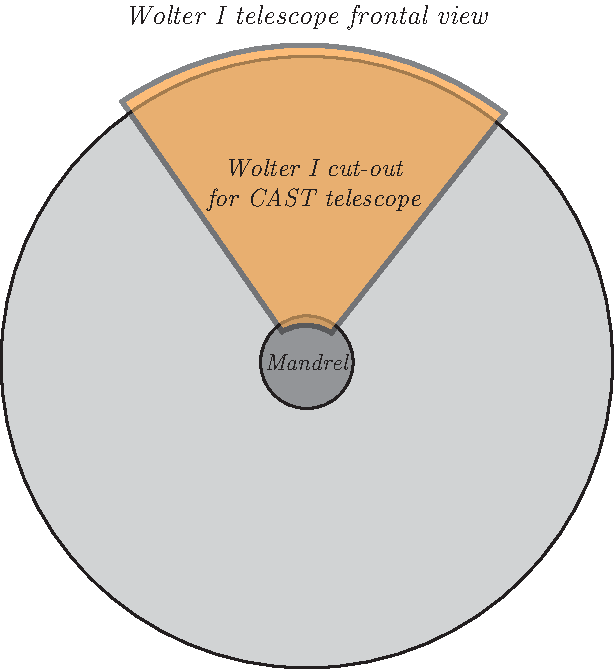
\includegraphics[width=\linewidth]{figures/cast/wolter1-cutout.pdf}
  \captionof{figure}{\footnotesize Front view of Wolter I type optic with section used in the CAST XRT shown.}
  \label{fig:wolter1-cutout}
\end{minipage}%
\hspace{20pt}
\begin{minipage}{.52\textwidth}
  \centering  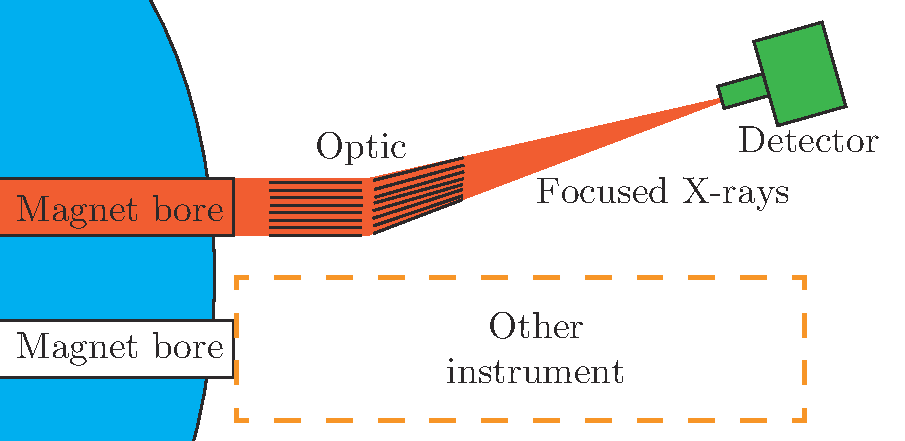
\includegraphics[width=\linewidth]{figures/cast/cast_xrt_principle.pdf}
  \captionof{figure}{\footnotesize Top-down view of the end of the CAST magnet, where an optic can be attached at one magnet bore. The other magnet bore is taken up by another instrument, resulting in limited space for the CAST XRT.}
  \label{fig:cast_xrt_principle}
\end{minipage}
\end{figure}
% \begin{figure}[htbp]
%   \centering
%     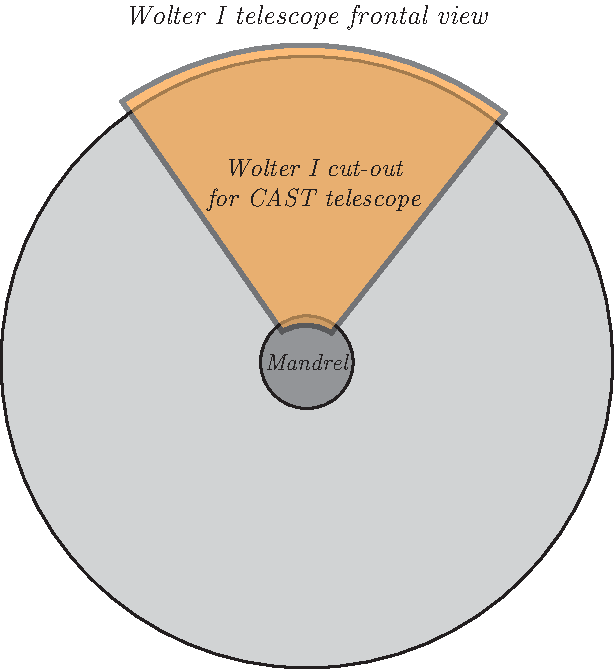
\includegraphics[height=5cm]{figures/cast/wolter1-cutout.pdf}
%     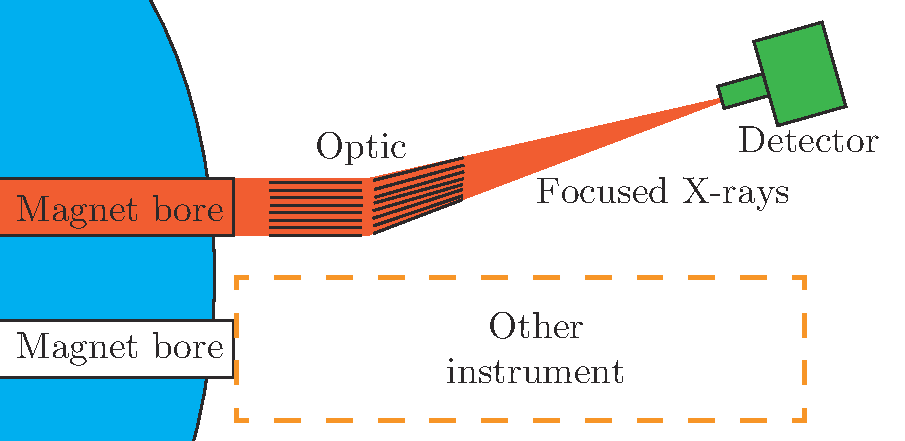
\includegraphics[height=5cm]{figures/cast/cast_xrt_principle.pdf}
%   \caption{\footnotesize Front view of Wolter I type optic with section used in the CAST XRT shown.}
%   \label{fig:wolter1-cutout}
% \end{figure}

By using only 1/6 of the Wolter I azimuthal area, a pie-slice (figure \ref{fig:wolter1-cutout}), two stacks of mirrors can be used to reflect X-rays to one side. The stack only needs to be high enough to cover the bore opening, but each mirror should also be wide enough. The NuSTAR glass pieces are made in 60\degr\ segments for the inner radii and 30\degr\ segments for the outer radii.

\subsection{Optic geometry considerations}
The geometry of the optic was calculated using the following equation for a Wolter I optic:
\begin{eqnarray}\label{eq:wolter}
  \tan(4\alpha) = \frac{\mathit{R3}}{f},
\end{eqnarray}
where $\alpha$ is the angle of reflection of each mirror, $f$ is the focal length and $\mathit{R3}$ is the radius between center of optic and the midpoint between parabolic and hyperbolic mirror (figure \ref{fig:wolter1-diagram}). The center of the bore will need an off-set with the focal plane of the telescope, given by $d = r_{\text{bore}} + r_{\text{min}}$, where $r_{\text{bore}}$ is the radius of the bore and $r_{\text{min}}$ is the minimum radius of a NuSTAR optic. The length of the NuSTAR mirrors is $l = 225$ mm.
% \begin{figure}
% \centering
% \begin{minipage}{.5\textwidth}
%   \centering
%   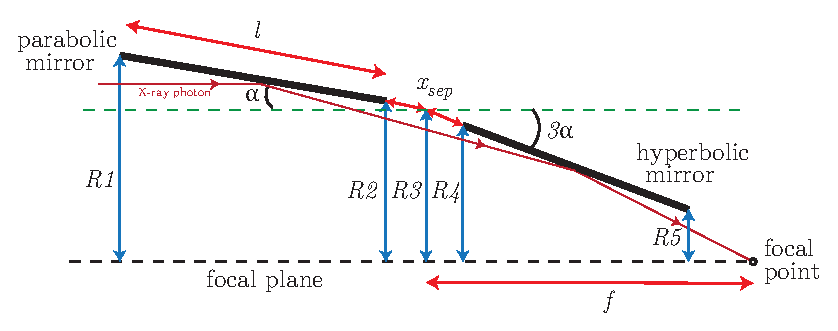
\includegraphics[width=\linewidth]{figures/cast/wolter1-diagram.eps}
%   \captionof{figure}{Diagram of wolter I from side.R1-R5 designated.}
%   \label{fig:wolter1-diagram}
% \end{minipage}%
% \begin{minipage}{.5\textwidth}
%   \centering  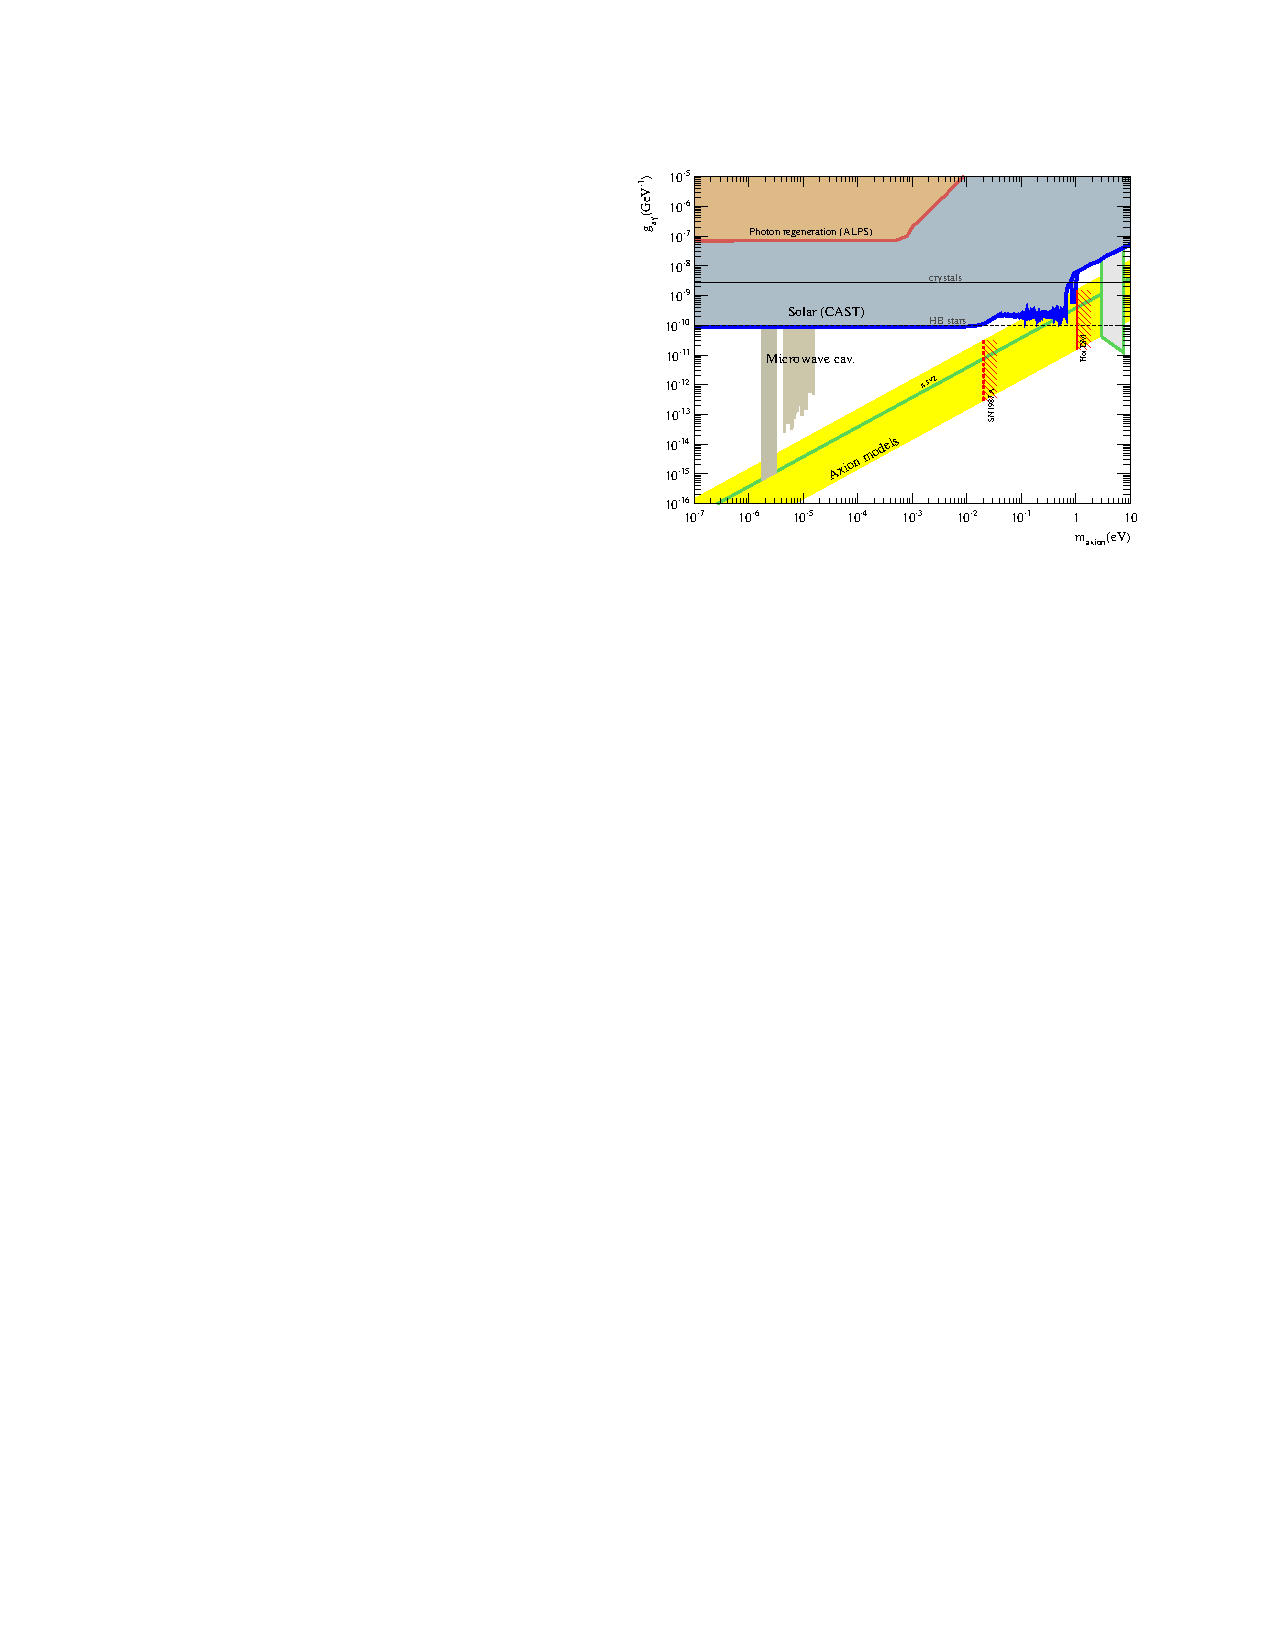
\includegraphics[width=\linewidth]{figures/cast/axion_search_cast.pdf}
%   \captionof{figure}{Show bore-opening with mandrel from front.}
%   \label{fig:optic_and_bore}
% \end{minipage}
% \end{figure}
\begin{figure}[htbp]
  \centering
    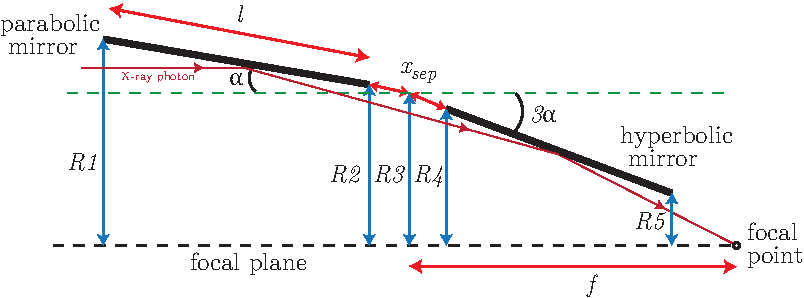
\includegraphics[width=0.95\linewidth]{figures/cast/wolter1-diagram.pdf}
  \caption{\footnotesize Diagram of Wolter I from side with $\mathit{R1}$-$\mathit{R5}$ designated. The principle of the Wolter I double reflection can be seen as an X-ray photon is reflected off the parabolic and hyperbolic mirrors. $l$ is mirror length, $f$ is focal length, $x_{sep}$ is distance between parabolic and hyperbolic mirror and $\alpha$ is the angle of reflection for an X-ray photon parallel to the focal plane.}
  \label{fig:wolter1-diagram}
\end{figure}

The focal length $f$ was set to a fixed value of 1.5 m. Using $r_{\text{min}}$ as the 0th layer radius, $\mathit{R3}_0$, the angle of the first layer, $\alpha_0$, can be calculated using eq. \ref{eq:wolter}. From $\alpha_0$ and $\mathit{R3}_0$, we can calculate $\mathit{R1}_0$, $\mathit{R2}_0$, $\mathit{R4}_0$ and \ensuremath{\mathit{R5}_0}:
\begin{eqnarray}
  \mathit{R2}_i &=& \mathit{R3}_i + 0.5\ x_{\text{sep}}\tan(\alpha_i),\\
  \mathit{R1}_i &=& \mathit{R2}_i + l\sin(\alpha_i),\\
  \mathit{R4}_i &=& \mathit{R3}_i - 0.5\ x_{\text{sep}}\tan(3\alpha_i),\\
  \mathit{R5}_i &=& \mathit{R4}_i - l\sin(3\alpha_i),
\end{eqnarray}
for layer $i=0$, where $x_{\text{sep}}$ is the distance between the parabolic and hyperbolic mirror. $\mathit{R4}_1$ and $\mathit{R5}_1$ will be a lower value than $r_{\text{min}}$, so it was nessecary to increase the bore to focal plane distance, $d$.

The next layer can be added by setting $\mathit{R3}_{i+1} = \mathit{R1}_i + d_{\text{glass}}$, where $d_{\text{glass}}$ is the thickness of the glass. Thereby the opening of the next layer will be exactly large enough for all incoming photons to hit the parabolic mirror. All mirror layers are subsequently added using the same method until the stack is high enough to cover the bore opening:
\begin{eqnarray}
  \mathit{R1}_{\text{last}} &\geq& r_{\text{min}} + 2r_{\text{bore}}.
\end{eqnarray}

\begin{figure}[htbp]
\centering
\begin{minipage}{.46\textwidth}
  \centering
  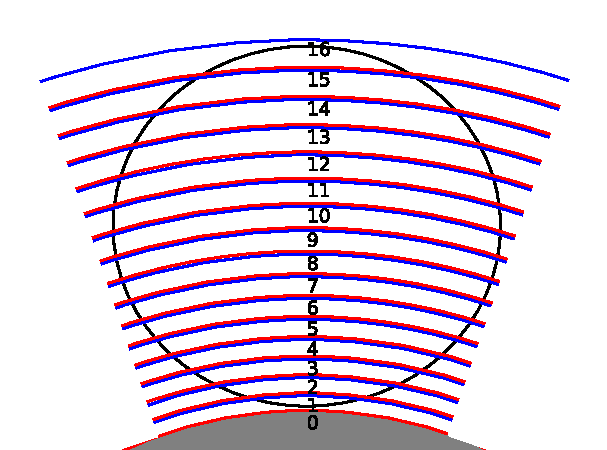
\includegraphics[height=4cm]{figures/cast/cast_front.pdf}
  \captionof{figure}{\footnotesize Computer generated CAST XRT design from front. Black ring designates the magnet bore opening.}
  \label{fig:cast_front}
\end{minipage}%
\hspace{20pt}
\begin{minipage}{.46\textwidth}
  \centering  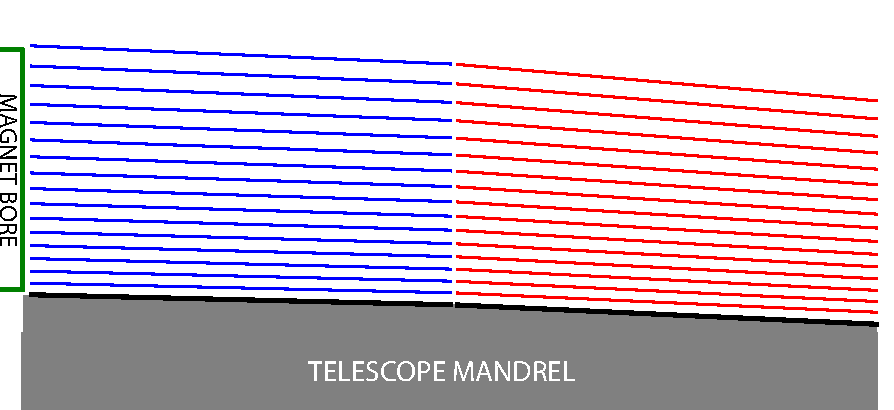
\includegraphics[width=\linewidth]{figures/cast/cast_side.pdf}
  \captionof{figure}{\footnotesize Computer generated CAST XRT design from side. Magnet bore opening is shown to the left.}
  \label{fig:cast_side}
\end{minipage}
\end{figure}

The calculated geometry can be seen in figure \ref{fig:cast_front} and \ref{fig:cast_side}. The calculated radius and angle for each layer can be seen in table \ref{tab:cast_geometry}. The area is the cross sectional area of the layer opening which overlaps with the magnet bore opening, a description of the calculation can be seen in section \ref{sec:eff_area}.

\begin{table}[!h]
\begin{center}
\begin{tabular}{c|c|c|c|c|c}
Layer & Area [mm$^2$] & $\alpha$ [\degr] & $\alpha$ [mrad] & $\mathit{R1}$ [mm] & $\mathit{R5}$ [mm]\\
\hline
%0&0.000&0.556&9.697&60.500&51.321 \\
1&13.863&0.579&10.113&63.006&53.821 \\
2&48.175&0.603&10.530&65.606&56.043 \\
3&69.270&0.628&10.962&68.305&58.348 \\
4&86.760&0.654&11.411&71.105&60.741 \\
5&102.266&0.680&11.877&74.011&63.223 \\
6&116.172&0.708&12.360&77.027&65.800 \\
7&128.419&0.737&12.861&80.157&68.474 \\
8&138.664&0.767&13.382&83.405&71.249 \\
9&146.281&0.798&13.921&86.775&74.129 \\
10&150.267&0.830&14.481&90.272&77.117 \\
11&149.002&0.863&15.062&93.902&80.218 \\
12&139.621&0.898&15.665&97.668&83.436 \\
13&115.793&0.933&16.290&101.576&86.776 \\
14&47.648&0.970&16.938&105.632&90.241
\end{tabular}
\end{center}
\caption{\footnotesize Geometric properties of the computer generated CAST XRT design. }\label{tab:cast_geometry}
\end{table}

Finally, we note that the actual radii and angles had to be slightly adjusted to allow the optic adhere to a cone-approximation to a true Wolter I design. These minor modifications to the radii and graze angles ensured the best possible focusing of the telescope and had negligible impact on multilayer optimisation.

\subsection{Optimising reflective coatings}\label{sec:opt_coatings}
To achieve the maximum possible efficiency of the optic, the coating needed to be optimised for the energy range. In contrast with most astrophysical observatories, the CAST telescope will only look at a single object with a very specific spectrum. That means that the coatings can be tailored to achieve maximum reflectivity in that area of the spectrum. Also known is the quantum efficiency of the detector.

An algorithm was developed to calculate all the different permutations of multilayers for a wide variety of material combinations. The spectrum is at a relatively low X-ray energy, so single layer coatings could be relevant. The algorithm calculates the reflectivity for a multilayer with given material combination and geometry at an angle, $\alpha$, given by the radius of the layer from the optical axis. $F.O.M.$ is then calculated using the following integral:
\begin{equation}\label{eq:fom}
	F.O.M. = \int_{0.1}^{10} \mathbb{R}^2(\mathrm{\alpha},\text{E})\ QE_{\text{det}}(\text{E})\ S_{\text{axion}}(\text{E})\ dE,
\end{equation}
with $\mathbb{R}^2(\mathrm{\alpha},\text{E})$ being the squared reflectivity because of the double reflection, $QE_{\text{det}}(\text{E})$ the detector quantum efficiency and $S_{\text{axion}}(\text{E})$ the axion spectrum as seen in figure \ref{fig:axion_spectrum}. By integrating over the energy range from 0.1 keV to 10 keV, a figure of merit can be obtained that takes both coating, spectrum and detector into account.

The material combinations considered were multilayers of W/B$_4$C, W/Si, Pt/C, Pt/B$_4$C, Ni/B$_4$C as well as single layers of W, Pt, Ir and Ni. W/Si and Pt/C were the most well understood for slumped glass type substrates, since they both were used in the NuSTAR mission. To find the optimal coating, the parameter space considered for each material combination can be seen in table \ref{tab:cast_parameter_space}. By using $d_{\text{min}}$ and $d_{\text{max}}$, both linearly graded-d coatings and constant-d coatings can be computed. To avoid computing cases where \(d_{\text{min}}\) is larger than \(d_{\text{max}}\), the condition \(d_{\text{min}}\) $\leq$ \(d_{\text{max}}\) was set.

\begin{table}[!h]
\begin{center}
\begin{tabular}{c|c|c|c}
Parameter & Minimum & Maximum & Interval \\
\hline
$N$ & 1 layer & 30 layers & 1 layer \\
$d_{\text{min}}$ & 3 nm & 300 nm & 0.5 nm \\
$d_{\text{max}}$ & 3 nm & 300 nm & 0.5 nm \\
$\Gamma$ & 0.1 & 0.9 & 0.05 \\
\end{tabular}
\end{center}
\caption{\footnotesize Parameter space used for finding optimal coating recipes for each material combination.}\label{tab:cast_parameter_space}
\end{table}

For single layer coatings, only a single thickness of 50 nm was considered. The surface and interface roughnesses were fixed at 0.5 nm. The complete computation can be done for every layer in the optic, as $\alpha$ changes throughout the mirror stack. The algorithm does the following steps:
\begin{itemize}
  \item[\bf 1] Finds the next combination in the parameter matrix.
  \item[\bf 2] Calculates the reflectivity using IMD's FRESNEL function.
  \item[\bf 3] Uses the calculated reflectivity in the $F.O.M.$ equation \ref{eq:fom}.
  \item[\bf 4] If the calculated value is higher than the previous maximum value, the parameters are saved and the calculated value set as the new maximum.
\end{itemize}

When the entire parameter space has been covered for a mirror layer and material combination, the algorithm saves the best $F.O.M.$ value and the coating recipe and goes on to the next mirror layer. When all mirror layers are covered, the effective area is calculated whereafter the algorithm continues on to the next material combination.

For the CAST coatings, making a separate coating recipe for each layer would result in having to produce $\sim$14 different coating runs, each with only four mirror substrates. Instead only four different coating recipes were made, where each recipe would be applied to three or four mirror layers. That way 16 mirror substrates could be coated at a time and all substrates could be coated in four coating runs. The result of a full computation using the algorithm with four recipes is shown in figure \ref{fig:mat_result}.

\begin{figure}[htbp]
  \centering
    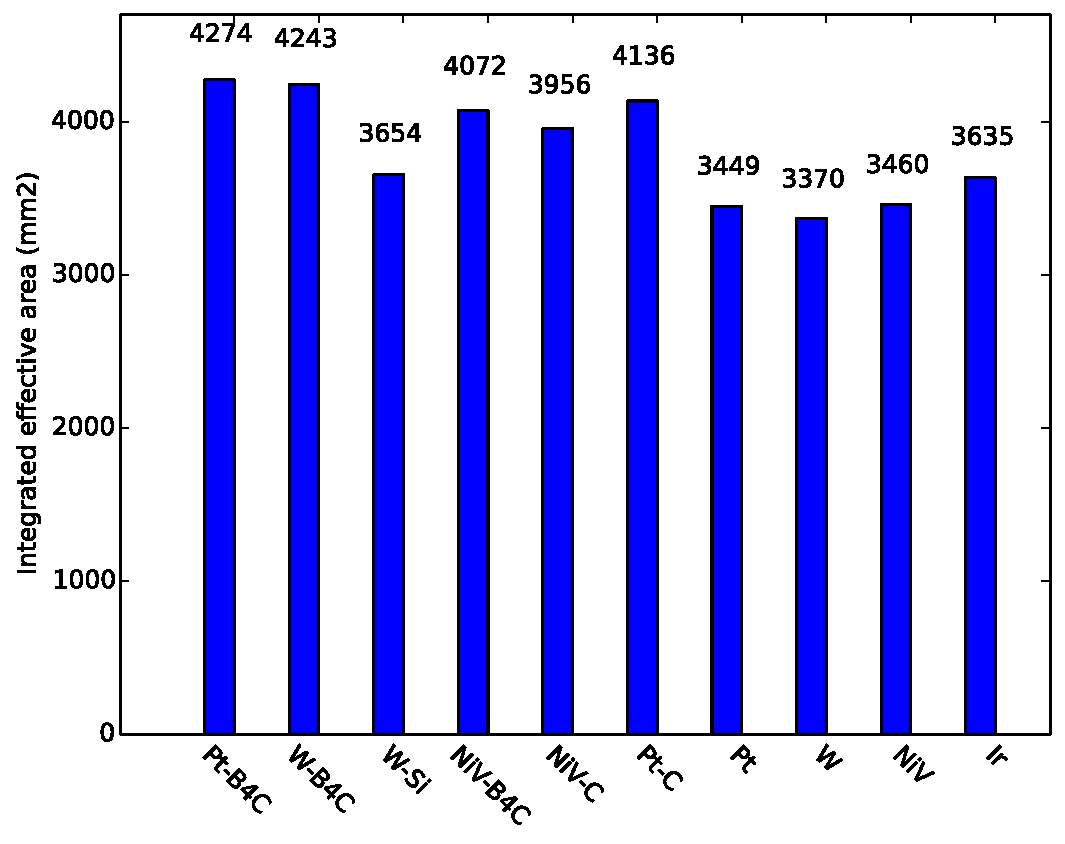
\includegraphics[height=5cm]{figures/cast/mat_result.pdf}
  \caption{\footnotesize Effective area comparison for computed material combinations in the CAST XRT optic.}
  \label{fig:mat_result}
\end{figure}

The best result for the Pt/C material combination can be seen in figure \ref{fig:pt-c_optimized_recipes}. Curves are the reflectivity squared times detector quantum efficiency times axion spectrum ($\mathbb{R}^2\cdot QE_{\text{det}}\cdot S_{\text{axion}}$) for a given recipe.

\begin{figure}[htbp]
  \centering
    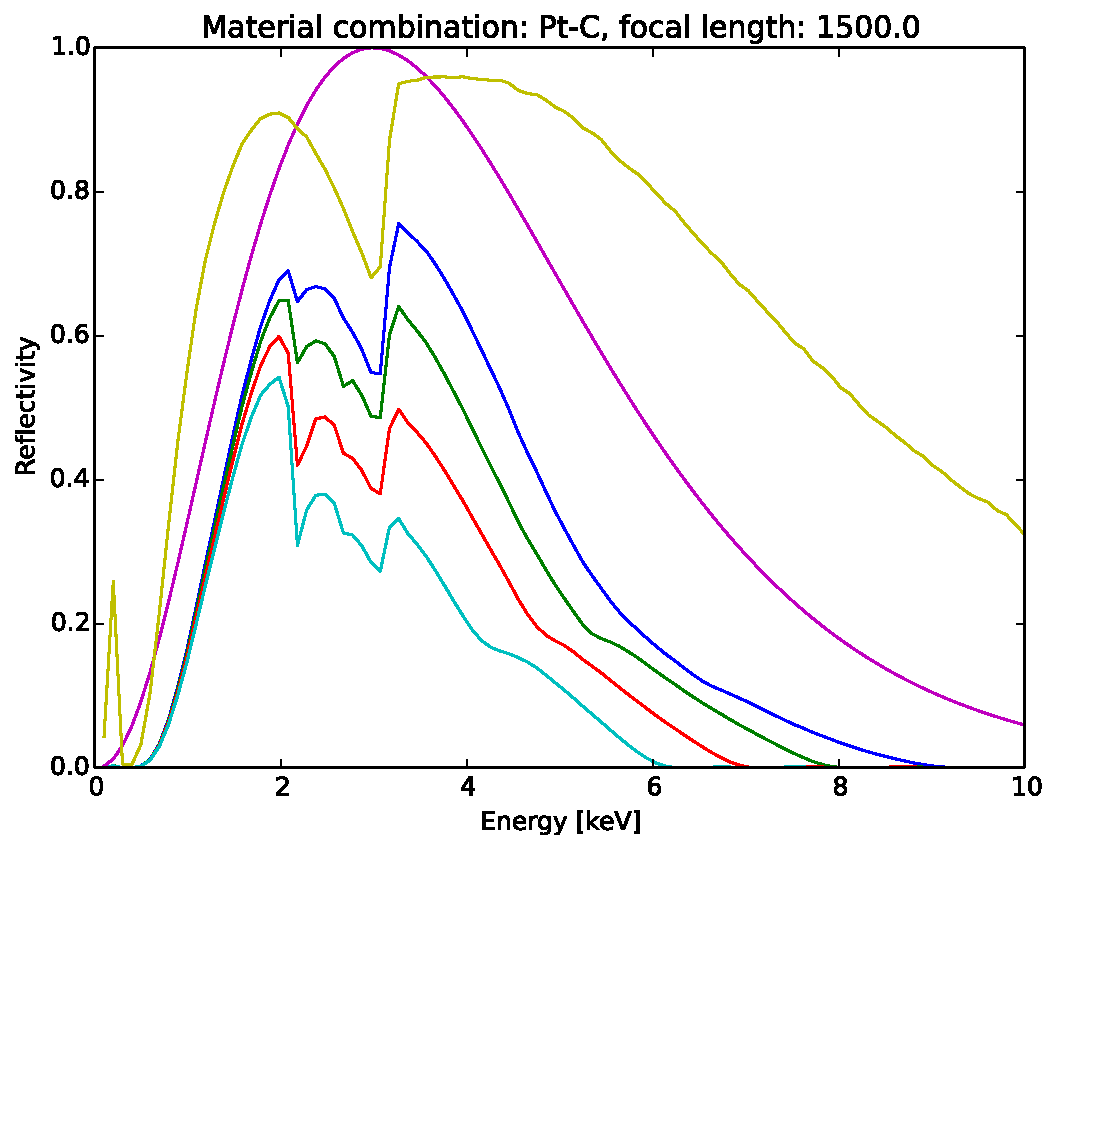
\includegraphics[height=5cm]{figures/cast/pt-c_optimized_recipes1.pdf}
    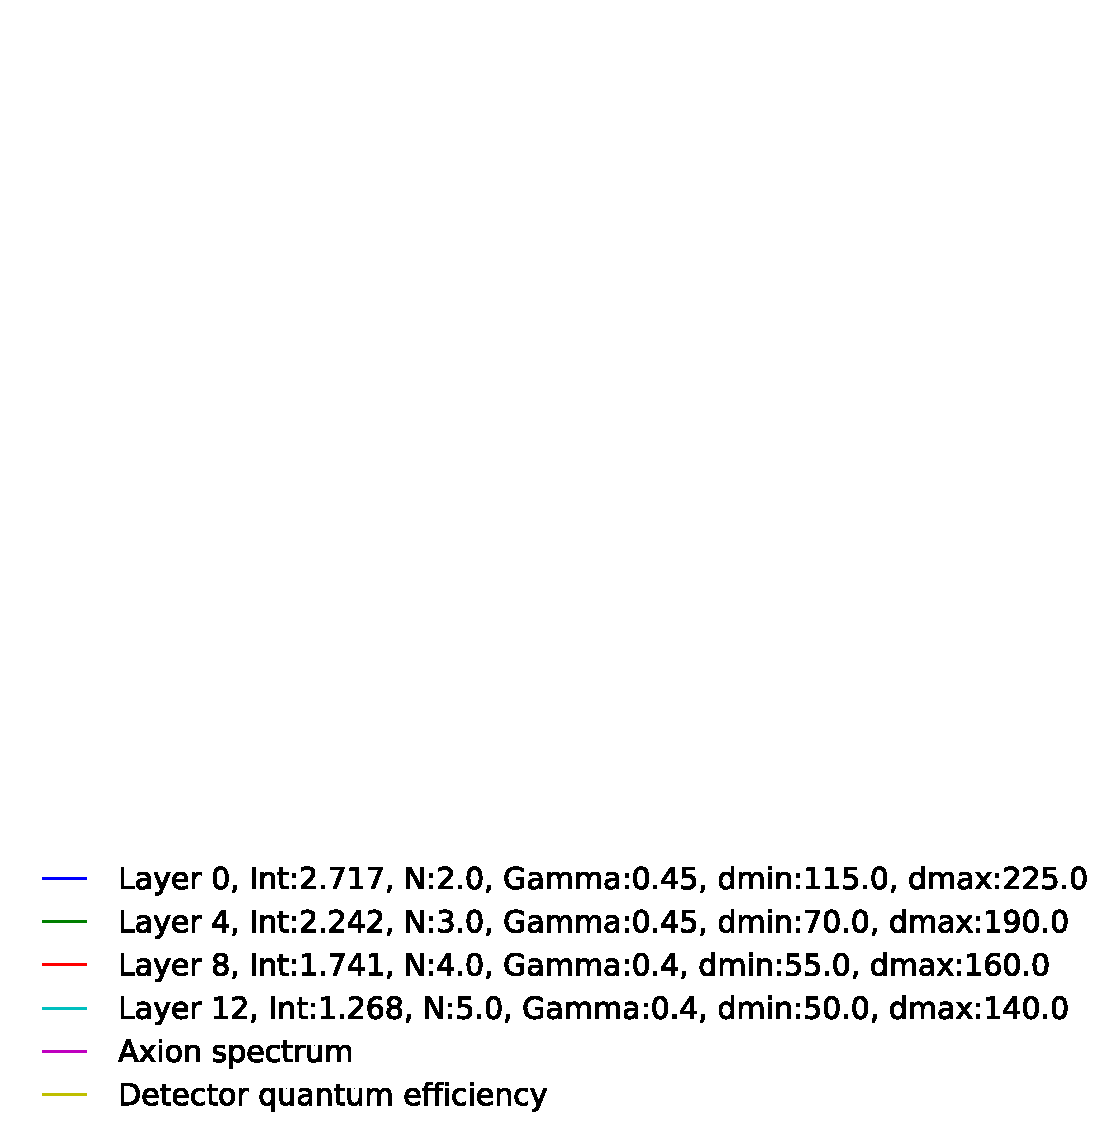
\includegraphics[height=1.5cm]{figures/cast/pt-c_optimized_recipes2.pdf}
  \caption{\footnotesize Optimised coatings for CAST XRT with a Pt/C material combination. The four recipes are for layer 0-3 (layer 0 is the mandrel), layer 4-7, layer 8-11 and layer 12-14.}
  \label{fig:pt-c_optimized_recipes}
\end{figure}

The coating optimisation for the CAST X-ray optic was done in parallel with most of the ATHENA coating investigations that is described in chapter \ref{chap:athena_coatings}. The findings from long term storage that are discussed in section \ref{sec:long_term} show changes in the coatings over time at ambient conditions for most B$_4$C containing films. For that reason, it was decided to make the CAST coatings with Pt/C, as the combination is well described for NuSTAR like glass substrates. W/Si was also used for NuSTAR and would be a cheaper solution, but the Si absorption line at $\sim2$ keV would decrease efficiency of the coatings around the peak of the axion spectrum.
%Each calculation was done over the energy range $0.1 - 10$ keV with a step size of 0.1 keV.

\subsection{Calculating effective area}\label{sec:eff_area}
The effective area is the cross sectional opening of the optic multiplied by reflectivity squared for each layer. Total effective area is the sum of effective area for each layer:
\begin{eqnarray}
  A_{\text{eff,i}} &=& A_{\text{CS,i}}\mathbb{R}_i^2(\text{E})\\
  A_{\text{eff}} &=& \sum_{i=0}^n A_{\text{eff,i}}
\end{eqnarray}
The cross sectional opening is the intersection of the circle of the bore opening and a layer opening. The layer opening is the cross sectional area between two circles of radius $\mathcal{R}_{i}$ and $\mathcal{R}_{i-1}$, where
\begin{eqnarray}
  \mathcal{R} = \mathit{R1}.
\end{eqnarray}
It can be calculated using the overlap of the outer shell of the layer opening and the bore opening. From that is subtracted the overlap of the inner shell of the layer opening with the bore opening as seen in figure \ref{fig:cross_section_area}.

\begin{figure}[htbp]
  \centering
    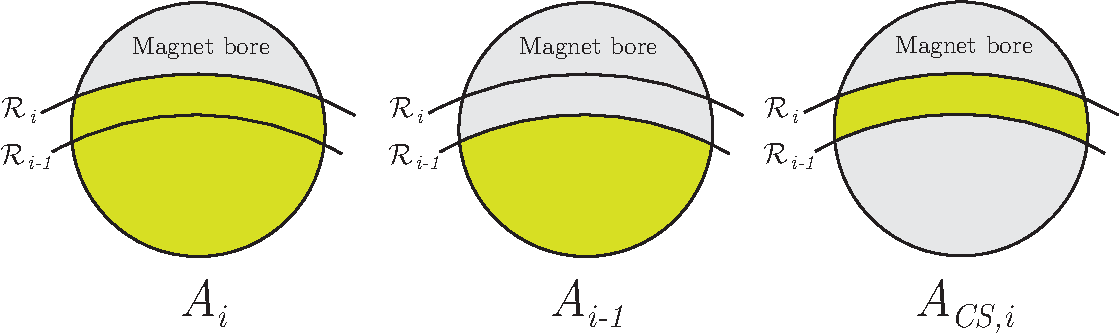
\includegraphics[width=0.9\linewidth]{figures/cast/cross_section_area.pdf}
  \caption{\footnotesize Diagram of cross sectional area (CSA) calculation for the intersection of the CAST XRT and CAST magnet bore. \textbf{Left:} CSA of layer $i$ and magnet bore. \textbf{Middle:} CSA of layer $i-1$ and magnet bore. \textbf{Right:} CSA between layer $i$, $i-1$ and magnet bore.}
  \label{fig:cross_section_area}
\end{figure}

Area of the overlap of shell $i$ with bore (figure \ref{fig:cross_section_area} left) is:
\begin{eqnarray}\label{eq:overlap1}
  A_{i} &=& r_{\text{bore}}^2\cos^{-1}\Big(\frac{d^2+r_{\text{bore}}^2-\mathcal{R}_{i}^2}{2dr_{\text{bore}}}\Big)\nonumber\\
  &&+\mathcal{R}_{i}^2\cos^{-1}\Big(\frac{d^2-r_{\text{bore}}^2+\mathcal{R}_{i}^2}{2d\mathcal{R}_{i}^2}\Big)\nonumber\\
  &&-\frac{1}{2}\sqrt{(-d+r_{\text{bore}}+\mathcal{R}_{i})(d+r_{\text{bore}}-\mathcal{R}_{i})}\nonumber\\
  &&\times\sqrt{(d-r_{\text{bore}}+\mathcal{R}_{i})(d+r_{\text{bore}}+\mathcal{R}_{i})},
  %A_{i-1} &=&
\end{eqnarray}
Area of the overlap of shell $i-1$ with bore (figure \ref{fig:cross_section_area} middle) is:
\begin{eqnarray}\label{eq:overlap2}
  A_{i-1} &=& r_{\text{bore}}^2\cos^{-1}\Big(\frac{d^2+r_{\text{bore}}^2-\mathcal{R}_{\text{bot}}^2}{2dr_{\text{bore}}}\Big)\nonumber\\
  &&+\mathcal{R}_{\text{bot}}^2\cos^{-1}\Big(\frac{d^2-r_{\text{bore}}^2+\mathcal{R}_{\text{bot}}^2}{2d\mathcal{R}_{\text{bot}}^2}\Big)\nonumber\\
  &&-\frac{1}{2}\sqrt{(-d+r_{\text{bore}}+\mathcal{R}_{\text{bot}})(d+r_{\text{bore}}-\mathcal{R}_{\text{bot}})}\nonumber\\
  &&\times\sqrt{(d-r_{\text{bore}}+\mathcal{R}_{\text{bot}})(d+r_{\text{bore}}+\mathcal{R}_{\text{bot}})},
\end{eqnarray}
where
\begin{eqnarray}\label{eq:overlap3}
  \mathcal{R}_{\text{bot}} &=& \mathcal{R}_{i-1} + d_{\text{glass}},
\end{eqnarray}
with $\mathcal{R}_{i-1}$ being the radius of the layer underneath layer $i$ and $d_{\text{glass}}$ being the thickness of the glass.

The NuSTAR type telescope is built up from glass layers with graphite spacers between.  Since the optic is so small, but with relatively large openings between the layers, it is necessary to use graphite spacers in the middle. Each of those are rectangular in shape, as high as the opening and $x_{\text{gr}}=2$ mm wide. The spacer obscures the opening, so will have to be subtracted from cross sectional opening. The cross sectional area of the  opening of layer $i$ is then:
\begin{eqnarray}
  A_{\text{CS,i}} &=& A_{i} - A_{i-1} - (\mathcal{R}_{i}-\mathcal{R}_{i-1})x_{\text{gr}}
\end{eqnarray}
The effective area and throughput for the optimised Pt/C coating can be seen in figure \ref{fig:pt-c_effarea_throughput}.

\begin{figure}[htbp]
  \centering
  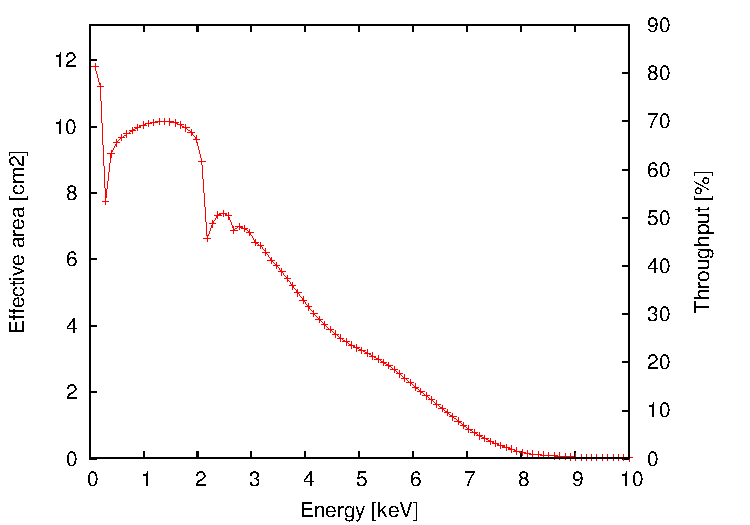
\includegraphics[width=0.47\linewidth]{figures/cast/pt-c_effara_throughput_lin.pdf}
  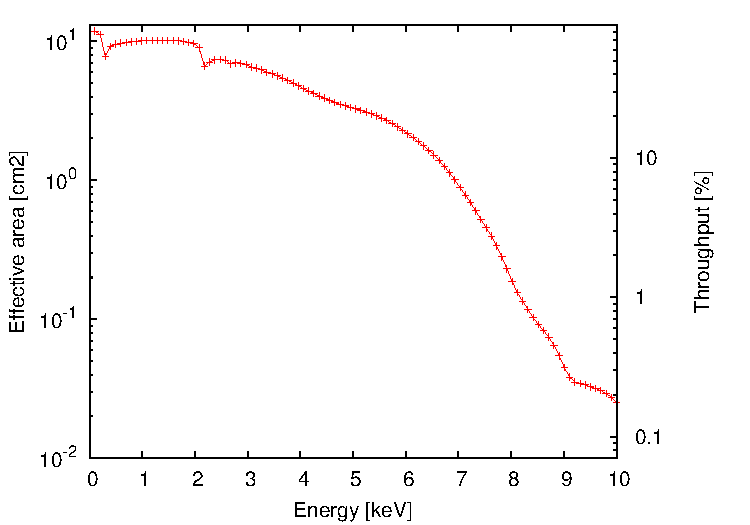
\includegraphics[width=0.47\linewidth]{figures/cast/pt-c_effara_throughput_log.pdf}
  \caption{\footnotesize Linear and logarithmic effective area curves of the CAST XRT given in cm$^2$. Throughput is given on the right side of each plot as the fraction of the magnet bore covered by the optic at a given energy.}
  \label{fig:pt-c_effarea_throughput}
\end{figure}

\section{Producing coated substrates}
DTU Space has a fairly large selection of leftover slumped glass substrates from the NuSTAR mission. An extra amount of glass substrates were produced to cover broken pieces and pieces that failed visual inspection. From this surplus, the substrates for the CAST XRT was selected.

\subsection{Collecting substrates for coating}
Each layer for NuSTAR corresponded to a shell diameter, which was described in the serial number of each substrate. The serial number includes diameter and wether it is a parabolic or hyperbolic piece. It is written with a marker on the back of the substrate like the following:
\begin{eqnarray}
  \text{NXXX(A/B)yyy-zzz(s/p),}\nonumber
\end{eqnarray}
where XXX is the diameter of the shell, (A/B)yyy describes the production batch of the slumped glass process, zzz is the layer number of the optic and (s/p) describes wether it is for the first or second stack (parabolic or hyperbolic). The NuSTAR optic is a conical approximation to the Wolter I geometry, but the glass substrates are produced on cylindrical mandrels. So instead of being parabolic or hyperbolic, they are straight along the optical axis.

To find pieces for the CAST XRT, the diameter described by XXX would need to correspond with the calculated $\mathit{R1}$ and $\mathit{R2}$ values for the first piece, or $\mathit{R4}$ and $\mathit{R5}$ for the second piece. The pieces should be mounted at higher grazing incidence angles than NuSTAR, so the difference between $\mathit{R1}$ and $\mathit{R2}$ are higher for CAST than NuSTAR. That difference would need to be corrected for by bending each piece to the correct shape during the mounting process. The NuSTAR pieces corresponding to the CAST radii can be seen in table \ref{tab:cast_pieces}.

\begin{table}[p]
\begin{center}
\begin{tabular}{c|c|c|c|c}
Layer & Mean diam. & Corresp. & Mean diam. & Corresp. \\
& (parabolic)  & NuSTAR & (hyperbolic)  & NuSTAR  \\
& [mm] &  diam. [mm] & [mm] &  diam. [mm]\\
\hline
1&124.2&124&114.7&116\\
2&129.3&128&119.5&120\\
3&134.7&136&124.4&124\\
4&140.3&140&129.6&128\\
5&146.0&144&134.9&136\\
6&152.0&152&140.5&140\\
7&158.3&160&146.2&148\\
8&164.8&164&152.2&152\\
9&172.5&172&158.4&160\\
10&178.4&180&164.8&164\\
11&185.7&184&171.5&172\\
12&193.2&192&178.5&180\\
13&201.0&200&185.7&184\\
14&209.1&208&193.1&192
\end{tabular}
\end{center}
\caption{\footnotesize Table of radii of each layer for the parabolic and hyperbolic mirrors in the CAST XRT compared to compatible NuSTAR radii.}\label{tab:cast_pieces}
\end{table}

\begin{figure}[htbp]
  \centering  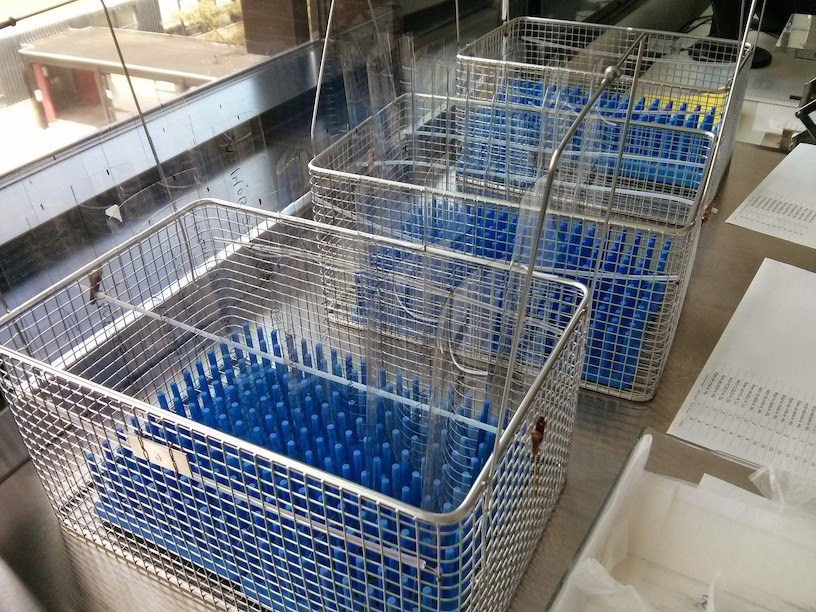
\includegraphics[height=6cm]{figures/cast/pieces_for_cleaning.jpg}
  \caption{\footnotesize Glass substrates selected for the CAST XRT before cleaning. The substrates required for each recipe were collected in four different baskets.}
  \label{fig:pieces_for_cleaning}
\end{figure}

With 14 glass layers and two stacks, 28 pieces are needed for the CAST XRT optic. As the glass pieces are very fragile and tend to break, it was decided to produce twice the amount, 56 in total.

Each piece was visually inspected and the best pieces were selected for the CAST XRT (figure \ref{fig:pieces_for_cleaning}). The pieces were subsequently cleaned by the following process:
\begin{enumerate}
  \item Ethanol rinsing to clear away markers.
  \item Clean room wipes were used to remove visible blemishes.\label{item:clean_wipes}
  \item 15 min. in ultrasonic bath with milli-Q water and soap (figure \ref{fig:cast_cleaning_soap}).
  \item Thorough rinse with milli-Q water to remove soap.
  \item 15 min. in ultrasonic acetone bath (figure \ref{fig:cast_cleaning_ethanol}).
  \item 15 min. in ethanol bath (figure \ref{fig:cast_cleaning_ethanol}).
  \item Each piece rinsed with milli-Q water and carefully dried with dry N$_2$.
  \item Visual inspection, if failed, repeat from step \ref{item:clean_wipes}.
\end{enumerate}

\begin{figure}[htbp]
\centering
\begin{minipage}{.46\textwidth}
  \centering
  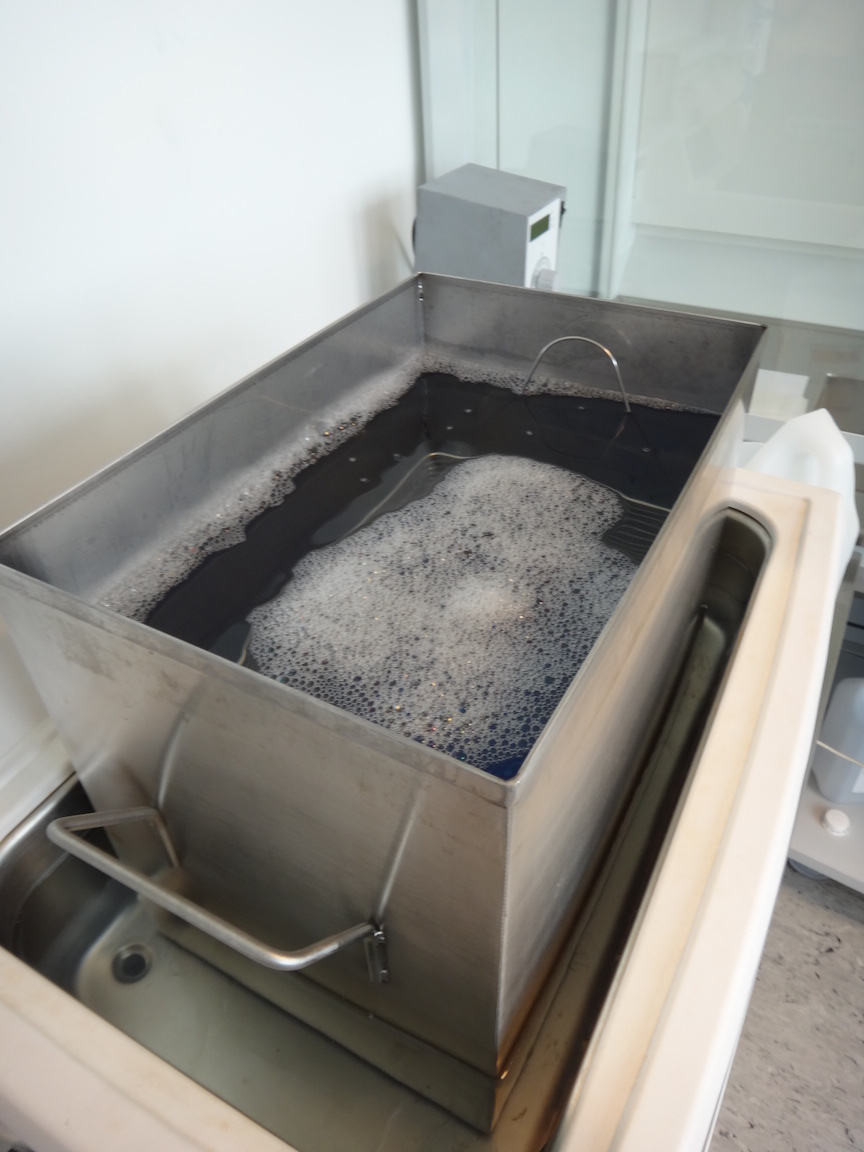
\includegraphics[height=4.5cm,trim= 0 100 0 200,clip]{figures/cast/soap_bath.jpg}
  \captionof{figure}{\footnotesize Ultra-sonic bath with soap.}
  \label{fig:cast_cleaning_soap}
\end{minipage}%
\hspace{20pt}
\begin{minipage}{.46\textwidth}
  \centering
  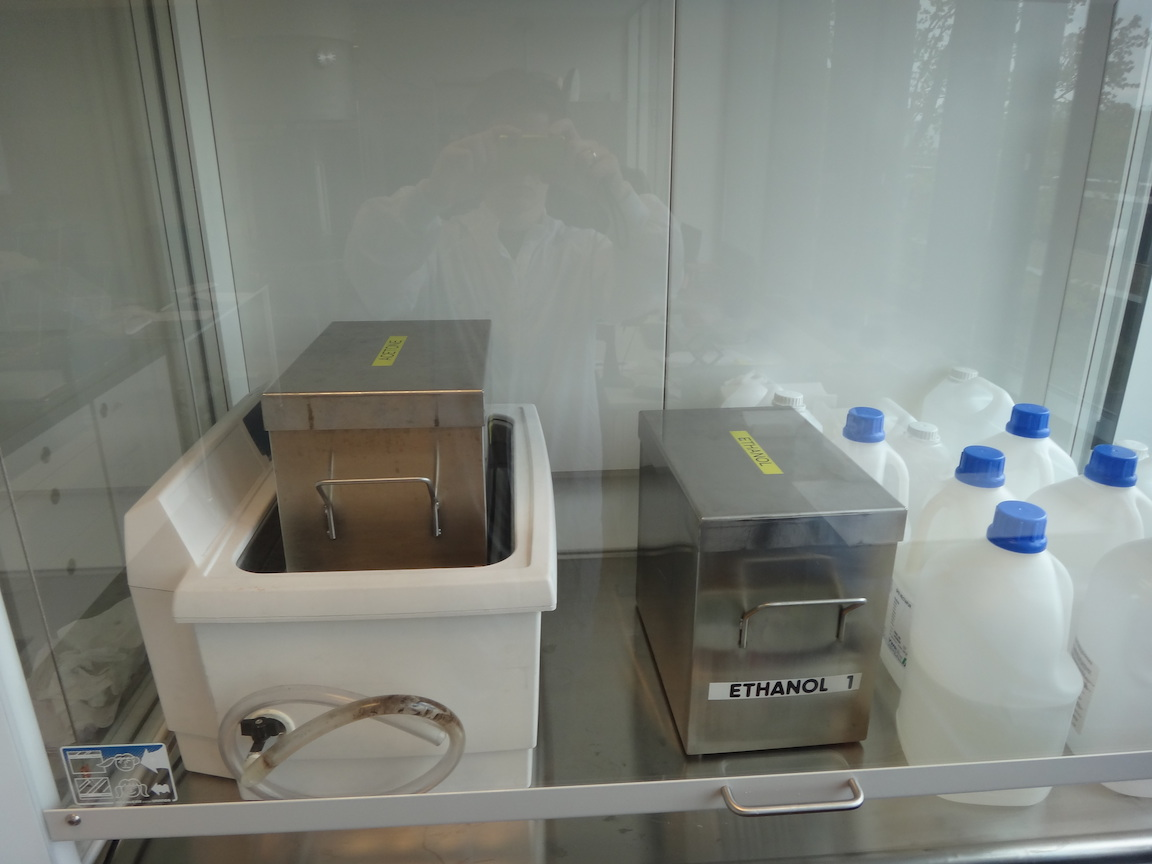
\includegraphics[width=0.9\linewidth]{figures/cast/acetone_and_ethanol.jpg}
  \captionof{figure}{\footnotesize Acetone and ethanol tubs. \textbf{Left:} Acetone tub in ultra-sonic machine. \textbf{Right:} Ethanol tub.}
  \label{fig:cast_cleaning_ethanol}
\end{minipage}
\end{figure}

The pieces were moved directly to sample mounting plates (figure \ref{fig:coating_mount}) in a downflow module to avoid dust contamination.

\begin{figure}[htbp]
  \centering
    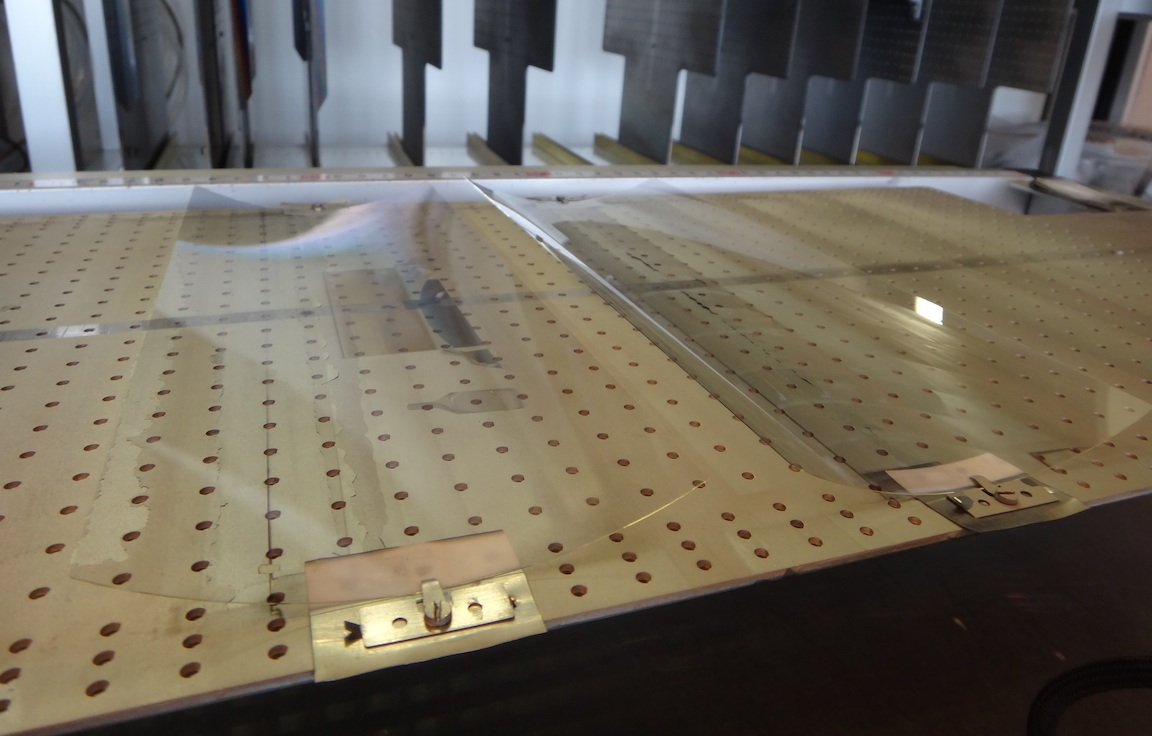
\includegraphics[height=6cm]{figures/cast/coating_mount.jpg}
  \caption{\footnotesize Cleaned glass substrates attached to sample mounting plate before coating. Two glass substrates were mounted onto each plate at positions 25 cm and 35 cm above coating chamber floor.}
  \label{fig:coating_mount}
\end{figure}

\subsection{Coating of substrates}
Four coating recipes were made for the CAST XRT. With 56 pieces to coat, 12-16 pieces are needed per recipe. The  coating chamber in the DTU Space multilab can hold up to 36 substrates if the entire length of each cathode is utilized. To ensure a uniform coating, only the center part of the coating cathodes are used. Two substrates were mounted on each plate so the center of each sample was 25 cm or 35 cm above the chamber floor. Along with the glass substrates, two Si wafer pieces were installed on a separate plate at the same height to become witness samples.

From the coating optimisation calculations described in section \ref{sec:opt_coatings}, the optimal material combination was chosen to be Pt/C. Before coating, a thorough calibration was needed, which was done as described in section \ref{sec:coating_calib}. Honeycomb (6.4 mm opening, 5 mm thickness) was used as collimation in front of the cathodes. A Pt target was mounted in cathode 2 and a 2-piece C target was mounted in cathode 4. Power settings were 450 W for cathode 2 and 900 W for cathode 4. Ar was supplied to the chamber at 88 SCCM, corresponding to a coating pressure of 2.9 mTorr. Background pressure for each coating was $\leq 2\cdot10^{-6}$ Torr.

\begin{figure}[htbp]
  \centering
    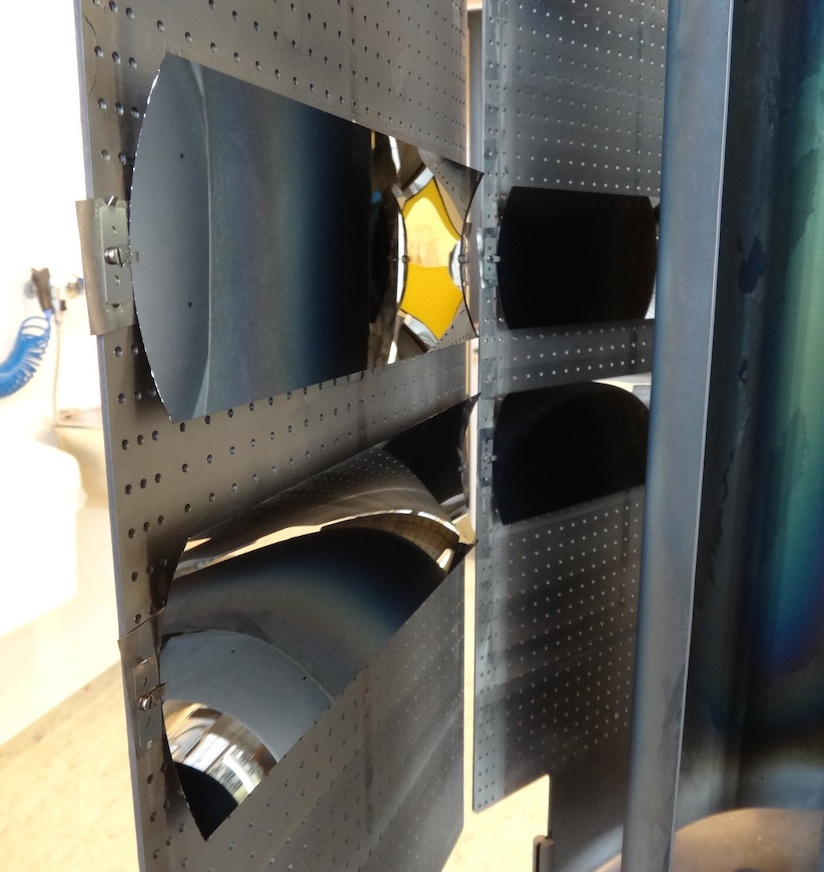
\includegraphics[height=7cm]{figures/cast/coated_pieces.jpg}
  \caption{\footnotesize Mounted glass substrates in coating chamber after coating. }
  \label{fig:coated_pieces}
\end{figure}

In figure \ref{fig:coated_pieces} can be seen the glass substrates after a coating still mounted in the coating chamber.

The coating was done with each material separately. With all cathodes turned off and the ring at the position where the first sample plate is between cathode 1 and 4, the ring would first move so sample plate 1 is next to the cathode of the first material. The cathode would then turn on, the shutter open and the ring start moving at the speed obtained from calibration corresponding to the thickness found in section \ref{sec:opt_coatings}. After one full rotation, the shutter closes, the cathode turns off and the ring returns to the start position before starting on the next material.

The power supplies were polled every 5 seconds to get the power output, which can be seen in figure \ref{fig:cast_coatings_power} for the coatings of recipe 1 and recipe 4. Cathode 5 and 6 are actually cathode 3 and 4 in the chamber, but are run from a third dual channel power supply. During the recipe 4 coatings can be seen some fluctuations in the cathode 4 power output, they are caused by the  instabilities that occur when coating with non-metallic materials at high power.

\begin{figure}[htbp]
  \centering  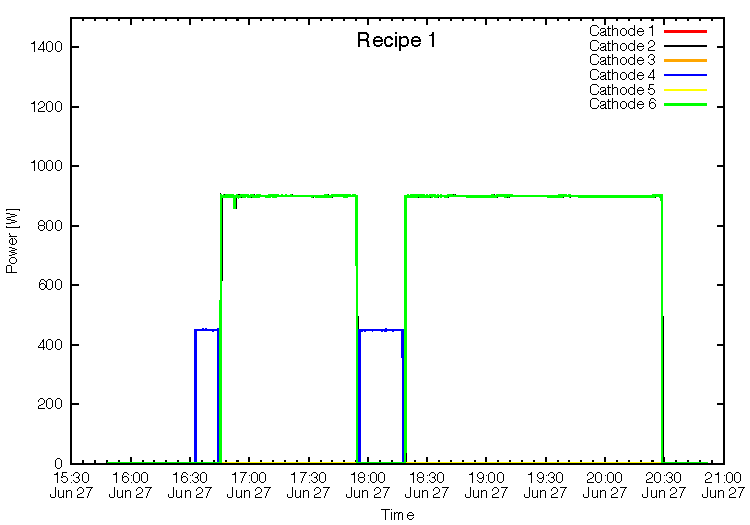
\includegraphics[width=0.45\linewidth]{figures/cast/power_recipe1.pdf}  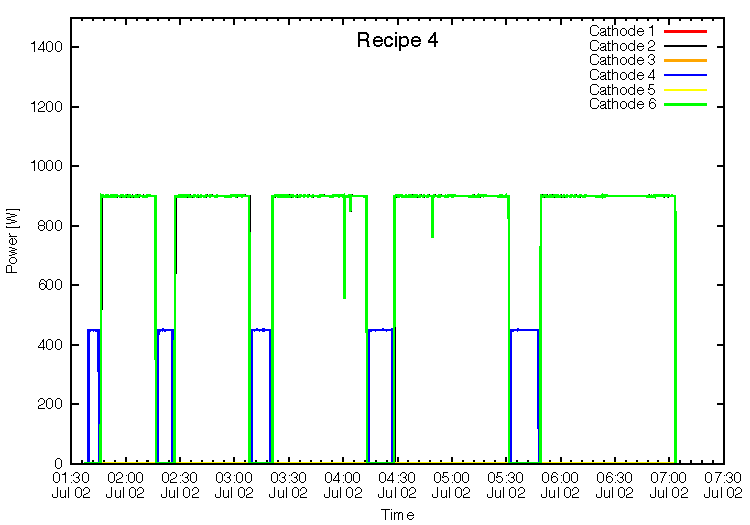
\includegraphics[width=0.45\linewidth]{figures/cast/power_recipe4.pdf}\\
  \caption{\footnotesize Graphs of power output delivered to cathodes from power supplies during CAST XRT multilayer coatings. \textbf{Left:} Cathode power output during recipe 1 coatings, two bilayers. \textbf{Right:} Cathode power output during recipe 4 coatings, five bilayers.}
  \label{fig:cast_coatings_power}
\end{figure}

The Si witness samples were measured at the XRR lab at DTU Space. XRR results from each witness sample for recipes 1-4 can be seen in figure \ref{fig:cast_recipe_xrr}. In each of the four coating runs, the two witness samples show completely similar XRR structure indicating a high uniformity between the two sample mounting positions. An exception is the witness samples from recipe 2, which show shifted peaks especially at higher angles as well as dissimilarities around the 5th peak.

\begin{figure}[htbp]
  \centering  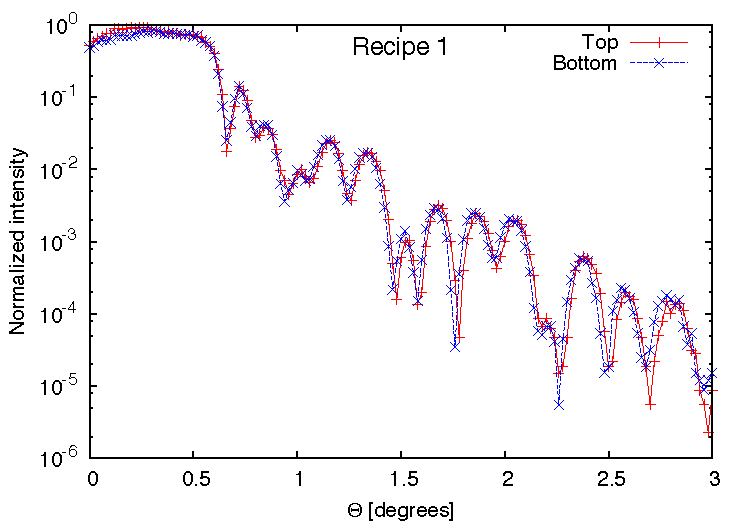
\includegraphics[width=0.45\linewidth]{figures/cast/cast_recipe1.pdf}  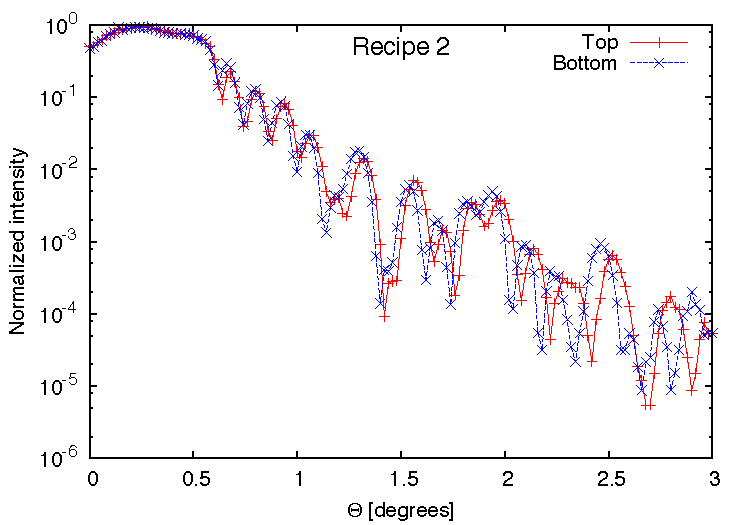
\includegraphics[width=0.45\linewidth]{figures/cast/cast_recipe2.pdf}\\  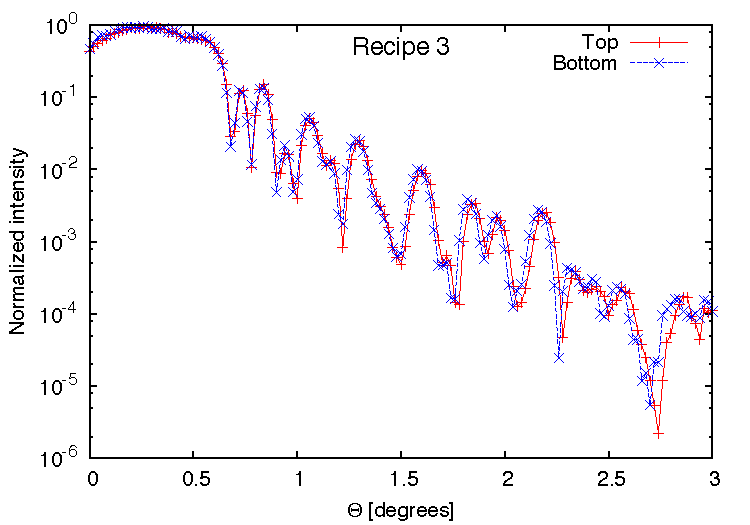
\includegraphics[width=0.45\linewidth]{figures/cast/cast_recipe3.pdf}  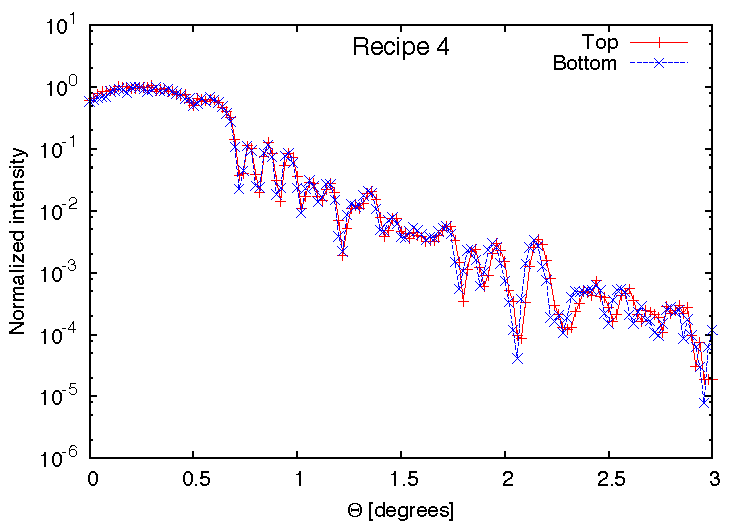
\includegraphics[width=0.45\linewidth]{figures/cast/cast_recipe4.pdf}
  \caption{\footnotesize XRR measurements of witness samples from CAST XRT coatings recipe 1-4. Each coating run included two witness samples placed at 25 cm and 35 cm above coating chamber floor, same as glass substrates.}
  \label{fig:cast_recipe_xrr}
\end{figure}

XRR data of witness samples were compared to an IMD model as seen in figures \ref{fig:cast_fit_rec1}, \ref{fig:cast_fit_rec2-1}, \ref{fig:cast_fit_rec2-2}, \ref{fig:cast_fit_rec3} and \ref{fig:cast_fit_rec4}. All fits show good agreement with XRR measurements despite the difficulties in fitting graded-d coatings as each layer thickness and interface roughness is an independent variable. All fits showed Pt/C and C/Pt interface roughness of $\sim$0.25--$\sim$0.35 nm.

\begin{figure}[h!]
\centering
\begin{minipage}{.47\textwidth}
  \centering
  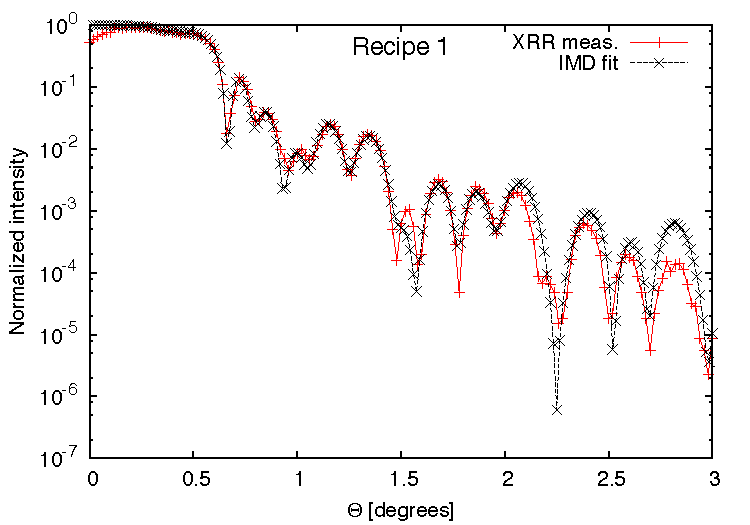
\includegraphics[width=\linewidth]{figures/cast/cast_recipe1_fit.pdf}
\end{minipage}%
\begin{minipage}{.53\textwidth}
  \centering
  \footnotesize
  \begin{tabular}{c|c|c|c|c}

i&d$_{\text{aim}}$ [nm]&$\Gamma_{\text{aim}}$&d$_{\text{fit}}$ [nm]&$\Gamma_{\text{fit}}$\\
  \hline
  1&22.5&0.45&22.48&0.462\\
  2&11.5&0.45&11.19&0.462
  \end{tabular}
\end{minipage}
\caption{\footnotesize XRR measurement of witness sample from CAST XRT recipe 1 coating compared to IMD model fit.}\label{fig:cast_fit_rec1}
\end{figure}

\begin{figure}[h!]
\centering
\begin{minipage}{.47\textwidth}
  \centering
  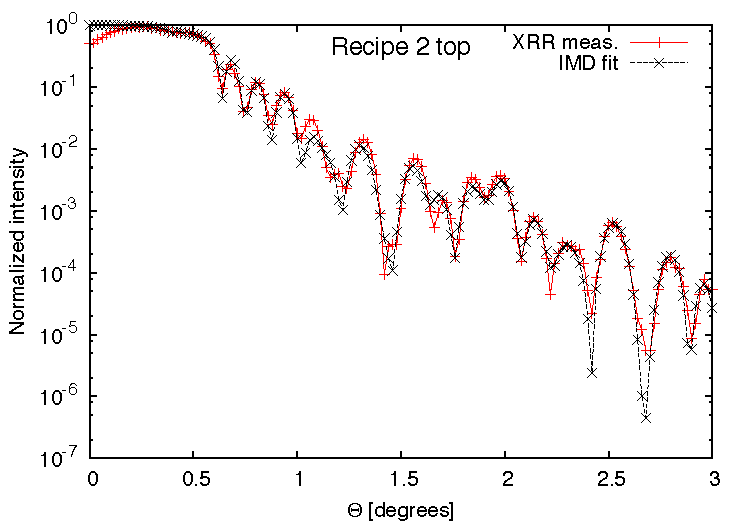
\includegraphics[width=\linewidth]{figures/cast/cast_recipe2_fit1.pdf}
\end{minipage}%
\begin{minipage}{.53\textwidth}
  \centering
  \footnotesize
  \begin{tabular}{c|c|c|c|c}
  i&d$_{\text{aim}}$ [nm]&$\Gamma_{\text{aim}}$&d$_{\text{fit}}$ [nm]&$\Gamma_{\text{fit}}$\\
  \hline
  1&19&0.45&18.53&0.46\\
  2&13&0.45&13.93&0.54\\
  3&7&0.45&6.89&0.46
  \end{tabular}
\end{minipage}
\caption{\footnotesize XRR measurement of witness sample from CAST XRT recipe 2 coating compared to IMD model fit. Witness sample was mounted 35 cm above coating chamber floor.}\label{fig:cast_fit_rec2-1}
\end{figure}

\begin{figure}[h!]
\centering
\begin{minipage}{.47\textwidth}
  \centering
  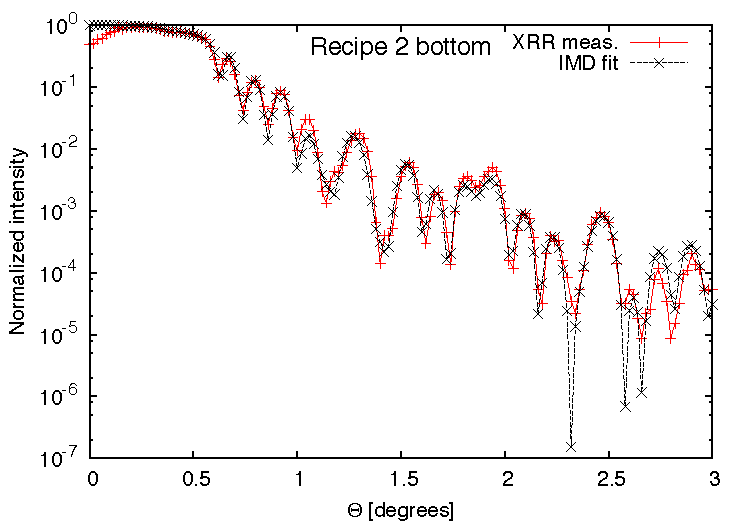
\includegraphics[width=\linewidth]{figures/cast/cast_recipe2_fit2.pdf}
\end{minipage}%
\begin{minipage}{.53\textwidth}
  \centering
  \footnotesize
\begin{tabular}{c|c|c|c|c}
i&d$_{\text{aim}}$ [nm]&$\Gamma_{\text{aim}}$&d$_{\text{fit}}$ [nm]&$\Gamma_{\text{fit}}$\\
\hline
1&19&0.45&18.40&0.448\\
2&13&0.45&14.57&0.558\\
3&7&0.45&6.99&0.449
\end{tabular}
\end{minipage}
\caption{\footnotesize XRR measurement of witness sample from CAST XRT recipe 2 coating compared to IMD model fit. Witness sample was mounted 25 cm above coating chamber floor.}\label{fig:cast_fit_rec2-2}
\end{figure}

\begin{figure}[h!]
\centering
\begin{minipage}{.47\textwidth}
  \centering
  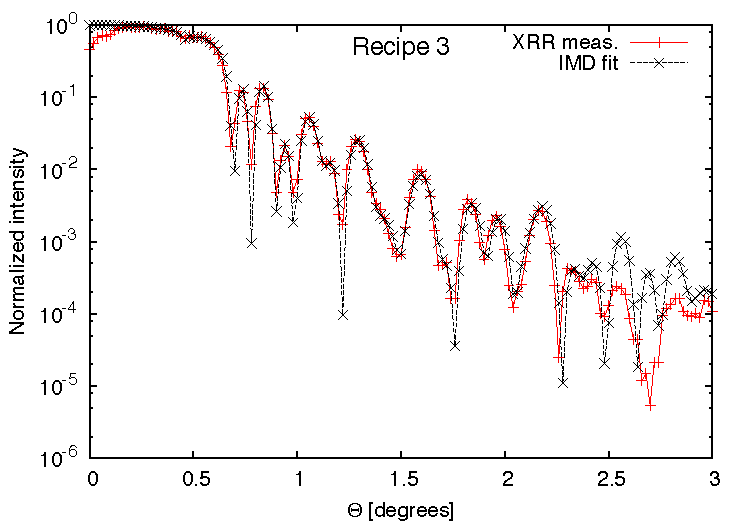
\includegraphics[width=\linewidth]{figures/cast/cast_recipe3_fit.pdf}
\end{minipage}%
\begin{minipage}{.53\textwidth}
  \centering
  \footnotesize
\begin{tabular}{c|c|c|c|c}
i&d$_{\text{aim}}$ [nm]&$\Gamma_{\text{aim}}$&d$_{\text{fit}}$ [nm]&$\Gamma_{\text{fit}}$\\
\hline
1&16&0.4&16.19&0.411\\
2&12.5&0.4&12.27&0.394\\
3&9&0.4&9.04&0.386\\
4&5.5&0.4&5.17&0.440
\end{tabular}
\end{minipage}
\caption{\footnotesize XRR measurement of witness sample from CAST XRT recipe 3 coating compared to IMD model fit.}\label{fig:cast_fit_rec3}
\end{figure}

\begin{figure}[h!]
\centering
\begin{minipage}{.47\textwidth}
  \centering
  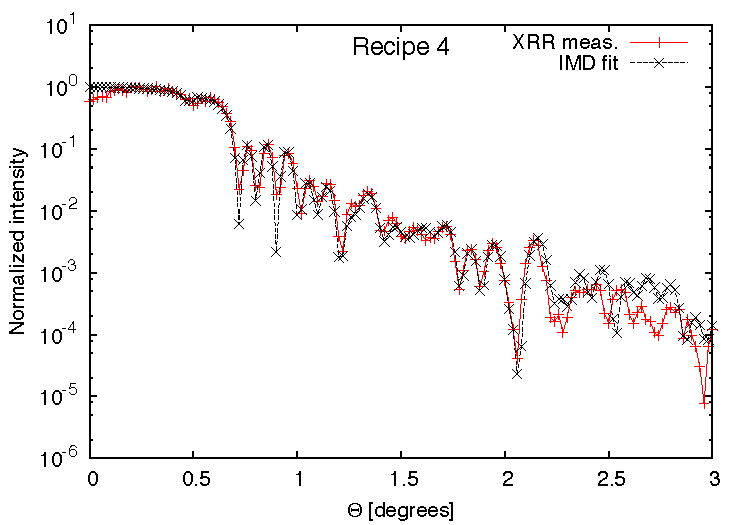
\includegraphics[width=\linewidth]{figures/cast/cast_recipe4_fit.pdf}
\end{minipage}%
\begin{minipage}{.53\textwidth}
  \centering
  \footnotesize
\begin{tabular}{c|c|c|c|c}
i&d$_{\text{aim}}$ [nm]&$\Gamma_{\text{aim}}$&d$_{\text{fit}}$ [nm]&$\Gamma_{\text{fit}}$\\
\hline
1&14&0.4&13.61&0.397\\
2&11.75&0.4&11.44&0.400\\
3&9.5&0.4&9.27&0.404\\
4&7.25&0.4&7.10&0.408\\
5&5&0.4&4.93&0.412
\end{tabular}
\end{minipage}
\caption{\footnotesize XRR measurement of witness sample from CAST XRT recipe 4 coating compared to IMD model fit.}\label{fig:cast_fit_rec4}
\end{figure}

Both top and bottom witness sample from the recipe 2 coatings were fitted given the dissimilarities stated above. The targeted coating for recipe 2 were 3 layers with d$_{\text{min}}=7$ nm, d$_{\text{max}}=19$ nm, $\Gamma=0.45$. Both top and bottom witness sample show a significant irregularity in the second bilayer where $\Gamma \simeq 0.55$ and d $\simeq$ 13.93-14.57 nm. The results warranted a thorough check of coating log and the coating macro used for the coating, as the irregularities could be at least partly explained by an error in the coating macro. No sign of error in the calculations of the coating macro, and the coating log also revealed that the speeds used during the coating corresponded to the values obtained in the calibration.

\begin{table}
  \centering
\begin{tabular}{c|c|c|c|c}
Witn. sample& d-C$_{\text{aim}}$ [nm]&d-C$_{\text{fit}}$ [nm]&d-Pt$_{\text{aim}}$ [nm]&d-Pt$_{\text{fit}}$ [nm]\\
\hline
Top&5.85&7.52&7.15&6.41\\
Bottom&5.85&8.13&7.15&6.44\\
\end{tabular}
\caption{\footnotesize Thicknesses of CAST XRT recipe 2 layer 2 in top and bottom witness sample, designed d-spacings from recipe compared to d-spacings obtained from XRR measurement and IMD fitting.}\label{tab:recipe2layer2}
\end{table}

The d-spacings for the second layer in recipe 2 compared to IMD fits of XRR data from top and bottom witness sample are shown in table \ref{tab:recipe2layer2}. An explanation for the inconsistencies between top and bottom witness sample could be problems with a cathode during coating. Column 3 shows inconsistencies between top and bottom witness sample in the C thickness, but it is not seen in the Pt thickness, column 5. That corroborates the hypothesis that the C cathode had difficulties during the application of the second layer, as indeed can be seen in figure \ref{fig:cast_coatings_power_recipe2_layer2}. The cathode is only polled every 5 seconds, so intermittent dropouts between polling are likely to have occurred. Top and bottom witness sample were mounted on the same plate, so passed the cathode simultaneously. The difference in C thickness can only be explained by a non-uniform coating rate of C during the coating of layer 2. A partial dropout of the C cathode could have put the power supply in a state where to reignite the plasma, the cathode would for some time have a non-uniform plasma density. Another explanation could be a localized charge-up on the C target during coating caused by the insulating properties of the material \footnote{The carbon targets used at DTU Space are boron-doped to increase the conductivity of the bulk material.}. Such a charge-up would change the electric field in front of the target and thereby create a non-uniform plasma density.

\begin{figure}[htbp]
  \centering  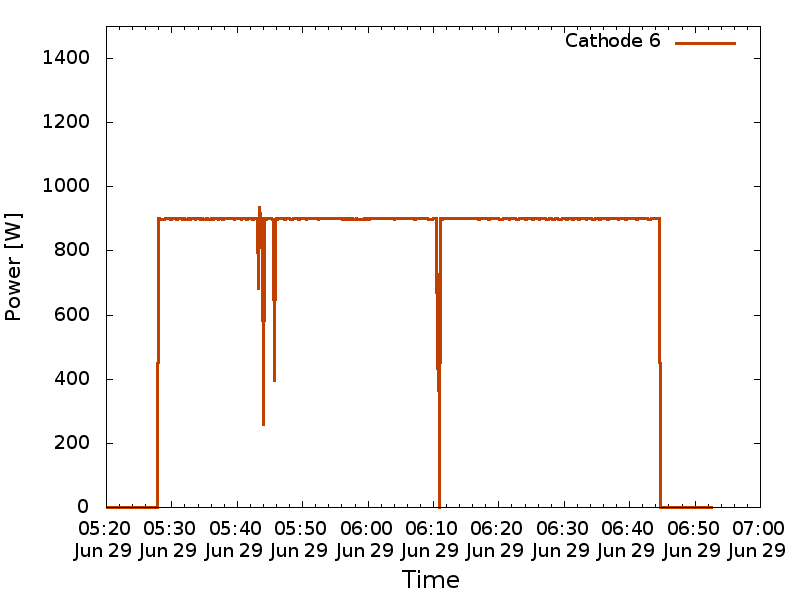
\includegraphics[width=0.7\linewidth]{figures/cast/power_cat6.png}
  \caption{\footnotesize Power output delivered to cathode 6 (carbon) during coating of layer 2, recipe 2. }
  \label{fig:cast_coatings_power_recipe2_layer2}
\end{figure}

The drop-outs of the C cathode can only explain the difference in C thickness between top and bottom witness sample. The inconsistencies of layer 2, recipe 2 is at the time of writing still of unknown origin.

The coated substrates were packed and shipped to LLNL for assembly.

\emph{The substrates were shipped with DHL, but the package was lost between Denmark and the US. A new batch of substrates were collected, cleaned, coated, packed and shipped during June/July of 2014. In this chapter is described the process for the second batch.}

\section{Assembling coated substrates}
Optic assembly was carried out at LLNL, where one of the NuSTAR assembly machines were set up for that purpose. The machine had been adjusted to make only a 30\degr\ section of substrates, and a specially designed Ti mandrel had been procured.

\begin{figure}[htbp]
  \centering
  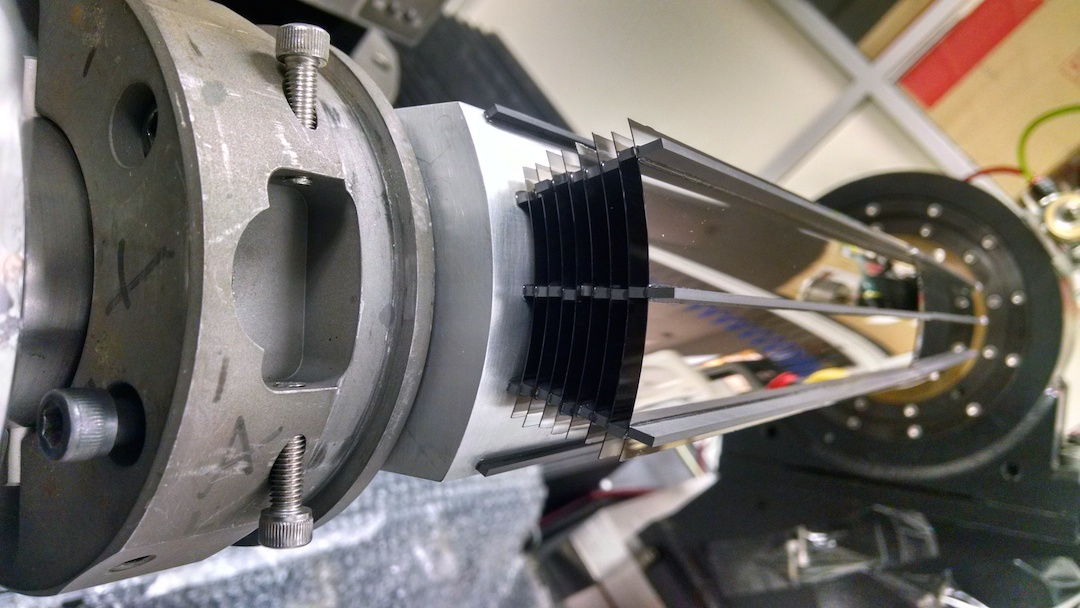
\includegraphics[width=0.45\linewidth]{figures/cast/assembly1.jpg}
  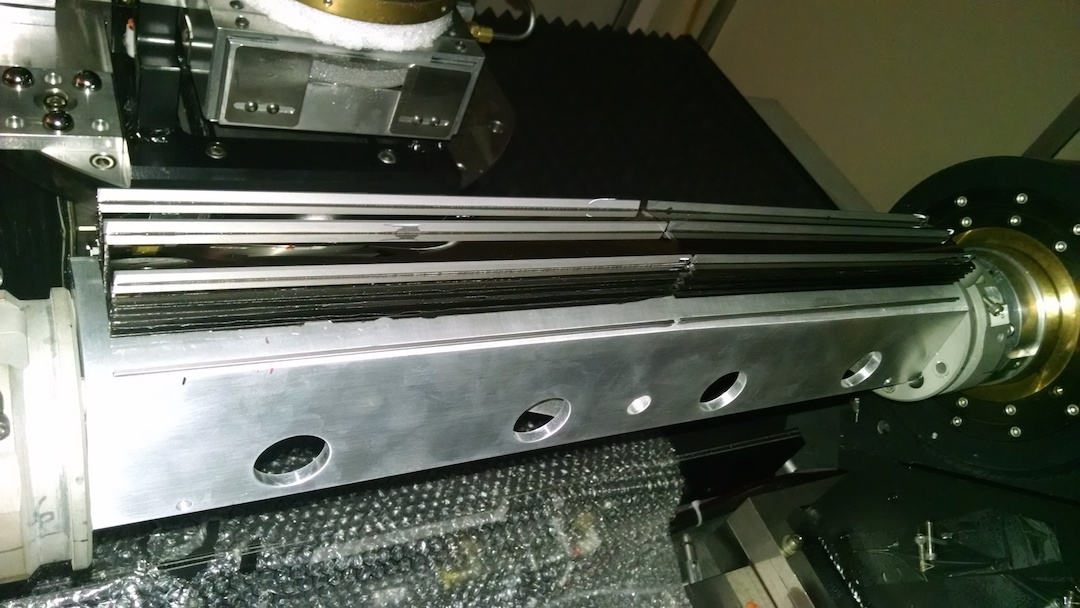
\includegraphics[width=0.45\linewidth]{figures/cast/assembly2.jpg}
  \caption{\footnotesize Pictures of glass substrates mounted on Ti mandrel during assembly. Three graphite spacers are attached on top of each glass substrate and machined to correct thickness before mounting of the next substrate.}
  \label{fig:cast_assembly}
\end{figure}

Three graphite spacers were mounted onto the mandrel with epoxy glue and machined to the correct thickness before the two pieces for the first layer were mounted, again using epoxy. The next set of graphite spacers were mounted onto the first glass substrates and then machined to the right thickness (figure \ref{fig:cast_assembly}).

\subsection{Vacuum vessel}
The magnet bores and detectors in the CAST helioscope operates at vacuum levels, so the entire optic had to be mounted inside a vacuum vessel. To align the optic after mounting it on the CAST helioscope, it was necessary to have linear actuators for the translation and rotation of the optic while under vacuum.

\begin{figure}[htbp]
  \centering
    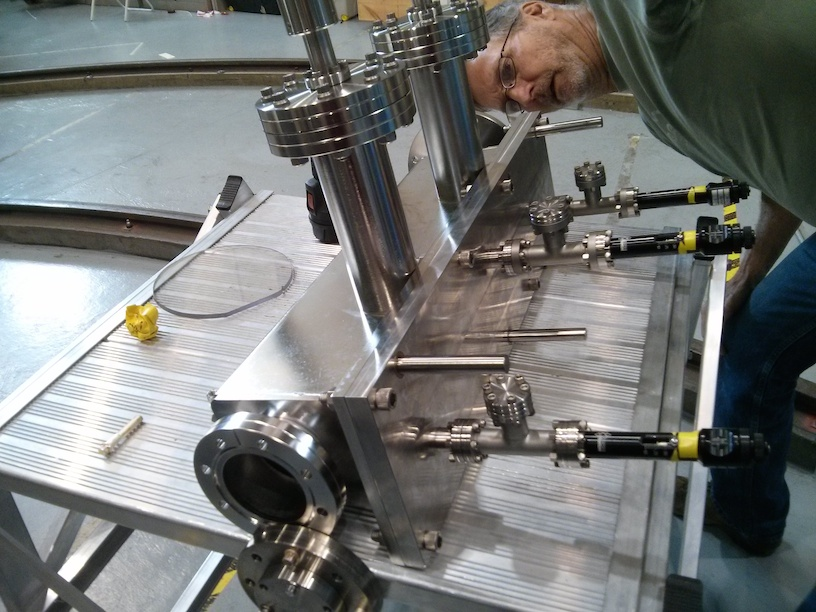
\includegraphics[width=0.45\linewidth]{figures/cast/cast_vessel1.jpg}
    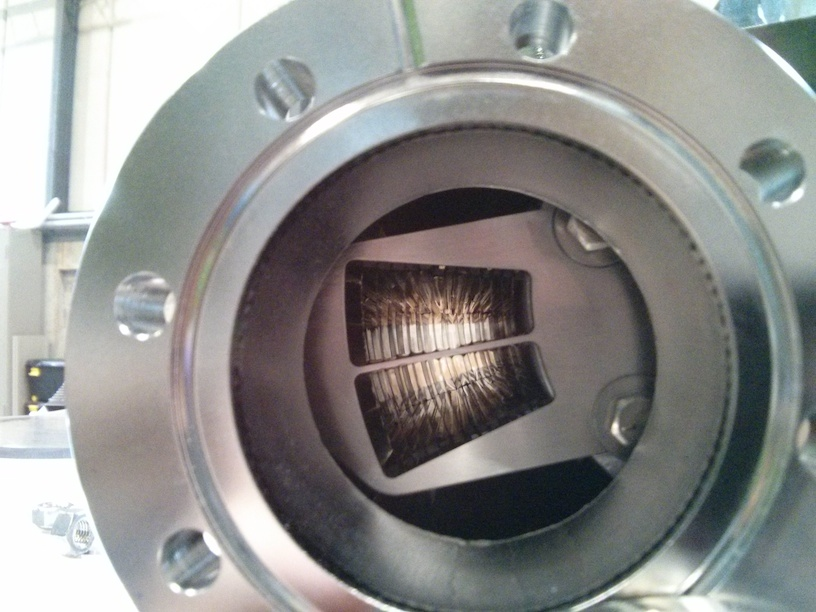
\includegraphics[width=0.45\linewidth]{figures/cast/cast_vessel2.jpg}
  \caption{\footnotesize Vacuum vessel for the CAST XRT. \textbf{Left:} Vacuum vessel with linear actuators and guide rods viewable. CF flange is mounted directly to the magnet. \textbf{Right:} Inside of vacuum vessel as viewed from CF flange. A metal plate with two openings cover the graphite spacers in the center between the glass layers. }
  \label{fig:cast_vessel}
\end{figure}

The vacuum vessel can be seen in figure \ref{fig:cast_vessel}. It was designed by Todd Decker (also pictured), an engineer from LLNL. In the picture can be seen five linear actuators, two on top to control pitch, three on the side, one for translation and two for yaw control. The three metal rods also visible on the side are for sliding out the optic, to make a precise optical alignment using a theodolite, described in detail in section \ref{sec:optic_alignment}.

Because of the limited space at the place where the optic had to be installed and the method of which to align it, the number of layers were cut from 14 to 13 layers. With 14 layers, the freedom of movement of the optic inside the vacuum vessel would have been severely limited and possibly caused the optic to hit the vacuum vessel wall during alignment.

\section{Installation of optic at CAST}
The optic mounted in the vacuum vessel was shipped to CERN for installation in Aug. 2014. The vessel was leak tested with He before being lifted into position in front of the magnet bore using a crane as seen in figure \ref{fig:cast_install}.

\begin{figure}[htbp]
  \centering
    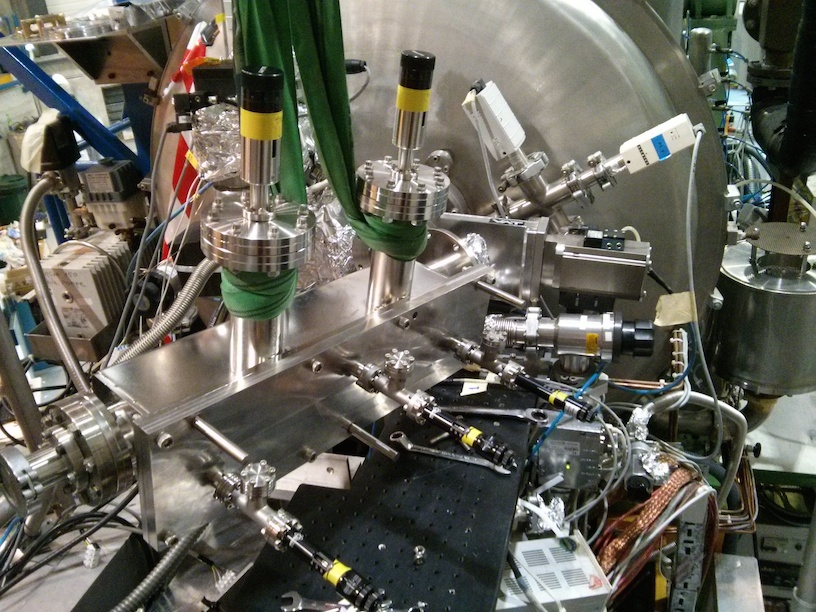
\includegraphics[height=6cm]{figures/cast/castxrt_install.jpg}
  \caption{\footnotesize The vacuum vessel housing the CAST XRT is lowered into place at the end of the CAST magnet using a crane.}
  \label{fig:cast_install}
\end{figure}

After mounting, vacuum view ports were mounted at either end of the magnet bores, making it possible to shine a laser straight through into the optic from the other end. The entire helioscope and magnet bore were also precisely aligned with a theodolite.

\subsection{Optic alignment}\label{sec:optic_alignment}
Inside the vacuum vessel, specially designed metal pieces were mounted to either end of the mandrel, one piece can be seen in figure \ref{fig:cast_vessel} (right). They have openings to allow photons into the optic and a narrow piece in the middle that blocks the graphite spacers between the glass pieces. Just above the top layer of glass was made a small hole in one of the metal pieces and on the other was mounted a small metal ball. The ball and hole were at the same distance from the center of the optic. The side of the vacuum vessel was designed so it could slide out a short distance along three precisely machined rods. By setting a pair of premachined spacers in the opening, the distance that the optic has slid out is exactly the distance from the hole and ball and the center of the optic.

A theodolite mounted 3 m from the front of the helioscope was aligned with the bore axis, so looking through the theodolite one could see the ball and hole of the optic. The optic rotation and translation could then be adjusted using the linear actuators to line up the ball and hole, and get a precise alignment. The theodolite could be set to shine a laser beam with adjustable divergence through the bore and at the optic. The view from the detector side can be seen in figure \ref{fig:ball_and_hole}. After the hole and ball was lined up, the optic was slid back into the vacuum vessel and the bolts were fastened.

\begin{figure}[htbp]
  \centering
    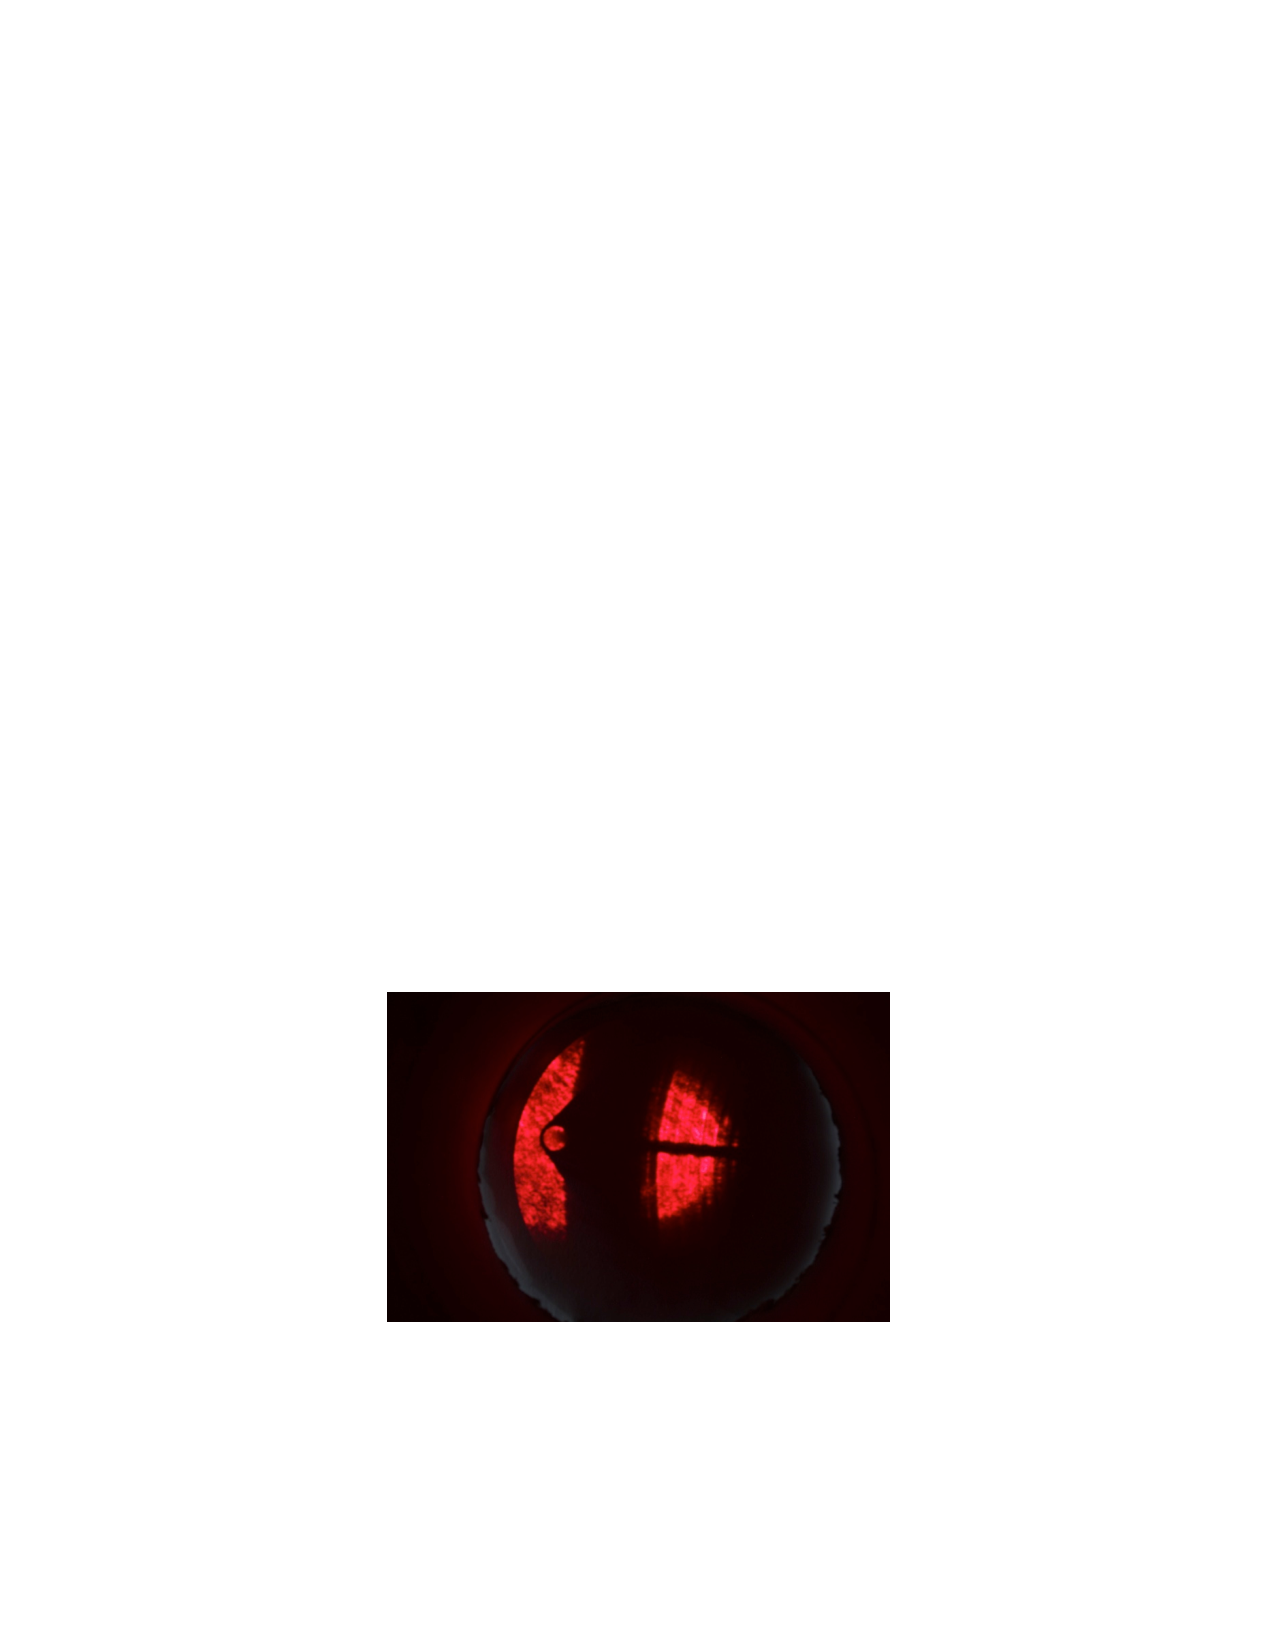
\includegraphics[height=4cm,trim=40 10 60 0, clip]{figures/cast/ballandhole.pdf}
    %\hspace{20pt}
    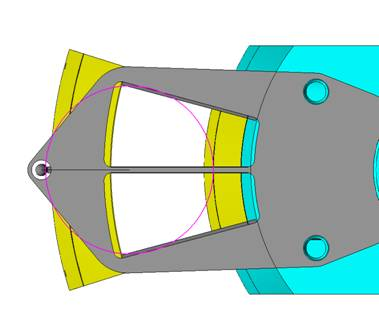
\includegraphics[width=0.47\linewidth]{figures/cast/ballandhole.jpg}
  \caption{\footnotesize \textbf{Left:} Picture taken from the detector side of the CAST XRT as a divergent laser beam shines through. A piece of paper covers the opening and is lit up by the laser. The optic has been moved out for alignment and the ball and hole are visible above the top glass layer. \textbf{Right:} CAD drawing of the CAST XRT with end-plates showing the ball and hole of the gunsight used for alignment (from Todd Decker, LLNL). }
  \label{fig:ball_and_hole}
\end{figure}

The optic reflected the laser light nicely, making it possible to get an exact position for the detector as seen in figure \ref{fig:cast_align} (left). A fake detector with a carbonite back was used for the alignment. That allowed the laser light focused by the optic to shine at the carbonite back and be viewable from the other side.

\begin{figure}[htbp]
  \centering
    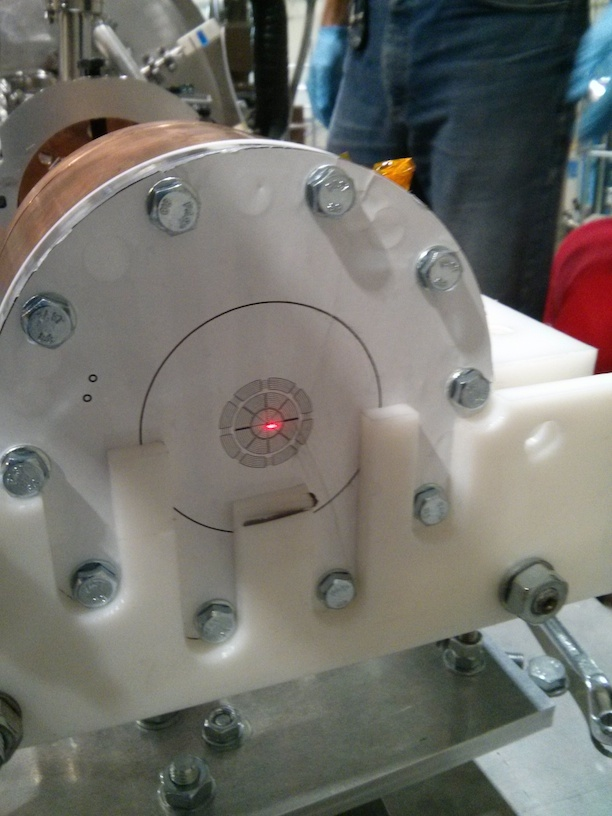
\includegraphics[height=5cm]{figures/cast/castxrt_alignment1.jpg}
    \hspace{20pt}
    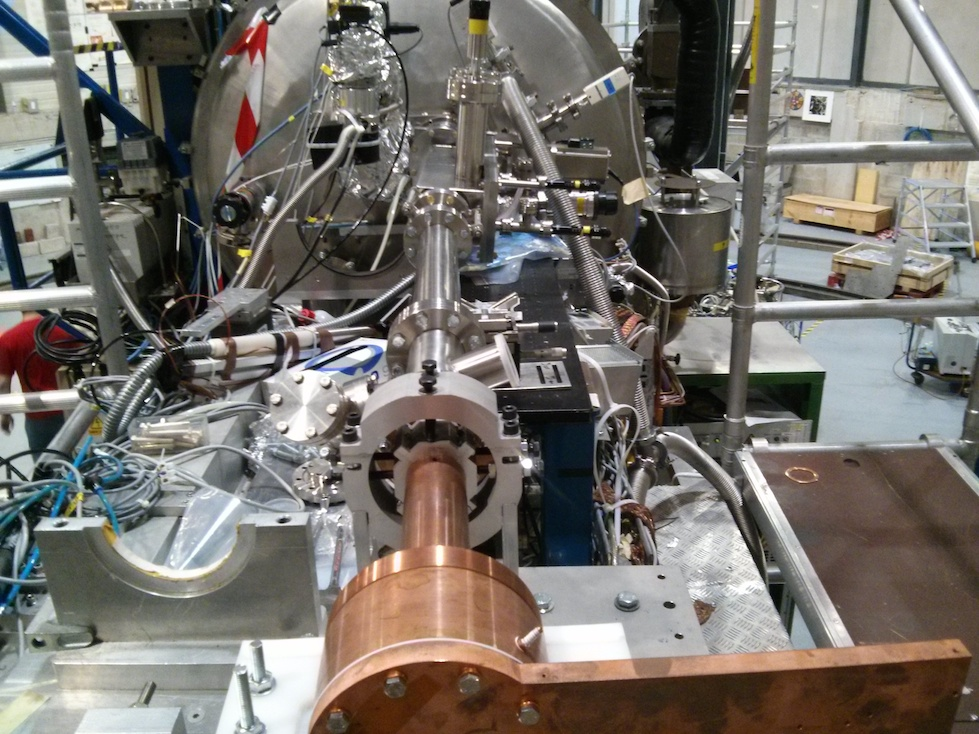
\includegraphics[width=0.45\linewidth]{figures/cast/castxrt_alignment2.jpg}
  \caption{\footnotesize MicroMegas detector alignment. \textbf{Left:} A fake detector with a carbonite back was installed. The divergent laser beam focused to a spot by the X-ray optic can be seen through the carbonite back. \textbf{Right:} The fake detector was exchanged for a functioning MicroMegas detector in the same mounting bracket and was connected to the vacuum system with XRT and magnet.}
  \label{fig:cast_align}
\end{figure}

The position of the detector was adjusted to make the spot hit in exactly the center. The detector mounts could then be fastened and the fake detector could then be replaced by a real one as seen in figure \ref{fig:cast_align} (right).

\subsection{Tests with 8 keV X-ray source}
The last task with detector and optic in place was a test with X-rays. An X-ray souce had to be mounted in front of the helioscope, but still under vacuum. It was decided to use a COOL-X pyroelectric X-ray source. It works by warming and cooling a pyroelectric element, which emits electrons that subsequently hits a Cu target, resulting in a bremsstrahlung spectrum and characteristic Cu emission lines. The source has a flux of $10^8$ photons/sec. emitted at an angle of 160\degr, so at a distance of $\sim$14.2 m from the optic, $<10$ photons/sec. would arrive at the detector on average given the integrated efficiency of the optic and the detector.

% \begin{figure}[htbp]
%   \centering
%     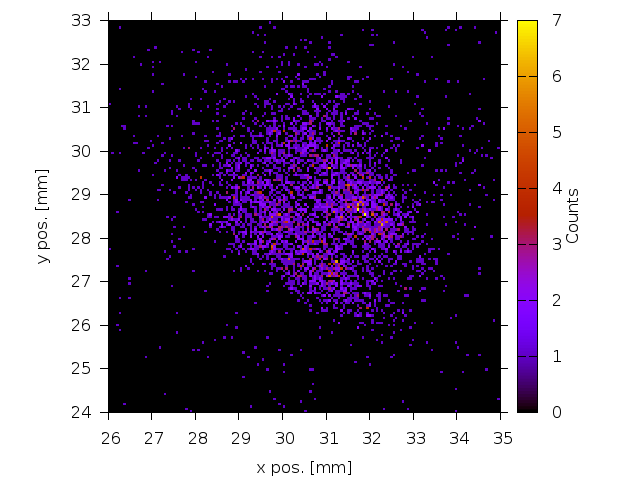
\includegraphics[width=0.47\linewidth,trim=40pt 0pt 30pt 0]{figures/cast/cast_5h_1000x.png}
%     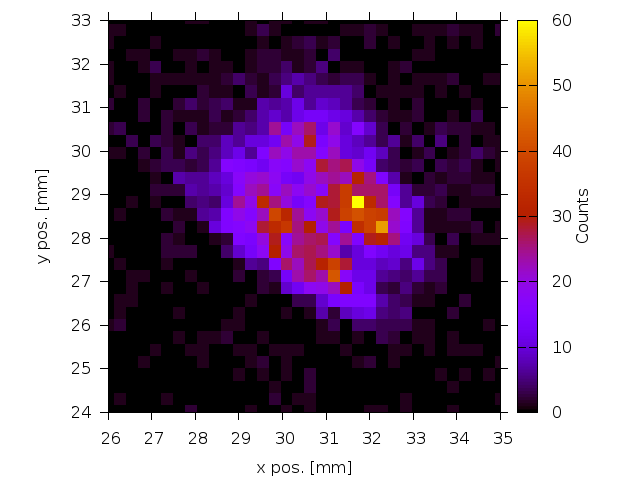
\includegraphics[width=0.47\linewidth,trim=40pt 0pt 30pt 0]{figures/cast/cast_5h_200x.png}
%   \caption{\footnotesize }
%   \label{fig:cast_5h_run}
% \end{figure}

%In figure \ref{fig:cast_5h_run} can be seen the data output from the MicroMegas detectors after a 5 hour measurement with the COOL-X X-ray source. Left figure is exact positions of each photon hitting the detector, right side shows the photons collected into bins, 200 bins per axis. The spot is $\sim$7 mm long and $\sim$5 mm wide, the relatively large spot is expected since the source is not a point source infinitely far away.
%A flux of less than 1 Hz was seen in the spot. According to the effective area plot in figure \ref{fig:pt-c_effarea_throughput}, the throughput at 8 keV is only $\sim$1\%.

Ray-tracing was done by Michael J. Pivovaroff from LLNL, and can be seen in figure \ref{fig:raytracing1}. The simulations assumes a 6 mm diameter source placed 14.2 m from the optic and glass figure errors comparable to the NuSTAR optic. The MicroMegas data from the 5 hour measurement was rotated 45 degrees and binned into 200 x 200 $\upmu$m$^2$ virtual pixels. By ray-tracing a 6 mm spot at discrete photon energies from 0-10 keV and using the measured spectrum as weight, a composite image was created to compare with measured data. The left plot of figure \ref{fig:raytracing1} is the ray-tracing and the right is the measured data with the ray-tracing model shown as red lines.

\begin{figure}[htbp]
  \centering
    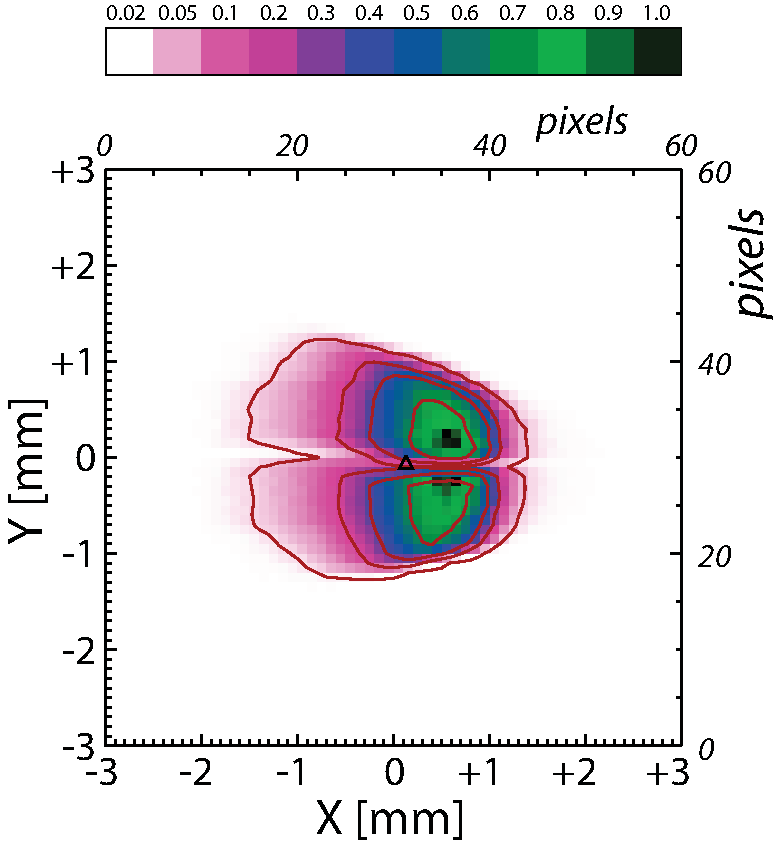
\includegraphics[width=0.47\linewidth]{figures/cast/coolX-simulation.pdf}
    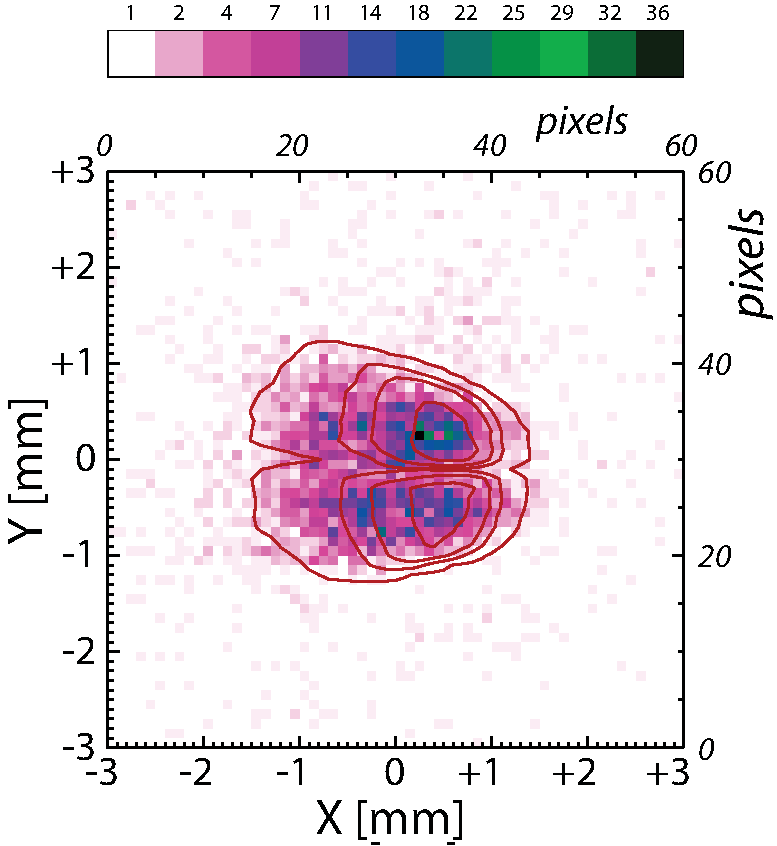
\includegraphics[width=0.47\linewidth]{figures/cast/coolX-SRMM.pdf}
  \caption{\footnotesize Comparison of ray-trace model with measurement using the COOL-X X-ray source.  \textbf{Left:} Ray-tracing simulation considering a 6 mm source 14.2 m from the optic.  \textbf{Right:} Measurement over 5 hours using the COOL-X X-ray source. White contours are from ray-tracing simulation. (From Michael J. Pivovaroff, LLNL) }
  \label{fig:raytracing1}
\end{figure}

Using the same model, a ray-tracing was done using a 3' source to mimic the helioscope looking at the sun and having axions converted into X-rays in the magnet. In figure \ref{fig:raytracing2} can be seen two ray-tracing models with a 3' source. Left plot assumes optic figure error of 1' (similar to NuSTAR) and right plot assumes optic figure error of 1.3'.

\begin{figure}[htbp]
  \centering
    \includegraphics[width=0.47\linewidth]{figures/cast/sunspot10.pdf}
    \includegraphics[width=0.47\linewidth]{figures/cast/sunspot13.pdf}
  \caption{\footnotesize Ray-trace model of CAST XRT considering the sun as a 3' source.  \textbf{Left:} Ray-tracing simulation considering optic with a figure error similar to NuSTAR of $\sim$1'.  \textbf{Right:} Ray-tracing simulation considering optic with a figure error 1.3 times greater than for NuSTAR ($\sim$1.3'). (From Michael J. Pivovaroff, LLNL) }
  \label{fig:raytracing2}
\end{figure}

The ray-tracing models show a half-power area of 8.6 mm$^2$ for the COOL-X X-ray source simulation , which corresponds well with the measurements seen in figure \ref{fig:raytracing1} (right). The measurements only lasted for 5 hours, so the photon count was relatively small because of the low flux from the source that actually reached the optic. The ray-tracing for a 3' source mimicking the sun show a half-power area of 1.44 mm$^2$. Had the optic figure been perfect (0'), the half-power area would be 1.39 mm$^2$, so the CAST XRT is close to the optimal performance.

In figure \ref{fig:raytracing3} can be seen the ray-tracing model computed for the as-designed multilayer coating (fig. \ref{fig:pt-c_optimized_recipes}) compared to the actual XRR measured and fitted multilayer coating (figures \ref{fig:cast_fit_rec1}--\ref{fig:cast_fit_rec4}). The as-coated multilayers differ in reflectivity response from as-designed multilayers by up to 0.5\% at the higher energies, at mid and lower energies the difference is less than 0.1\%. At higher energies, the effective area of the CAST XRT is  $< 10^{-1}$ cm$^2$ so changes in effective area become more pronounced.

\begin{figure}[htbp]
  \centering
    \includegraphics[width=0.47\linewidth]{figures/cast/raytracing_diff_cm2.pdf}
    \includegraphics[width=0.47\linewidth]{figures/cast/raytracing_diff_perc.pdf}
  \caption{\footnotesize Difference in the ray-trace model between as-designed multilayer coatings and actual XRR measured and fitted multilayer coatings.  \textbf{Left:} Difference in cm$^2$. \textbf{Right:} Difference in \% from actual effective area. (From Michael J. Pivovaroff, LLNL) }
  \label{fig:raytracing3}
\end{figure}

\section{Conclusion}
In this chapter was shown the creation of an X-ray optic from design phase to installation. The whole process was $\sim$2 years from start to finish and realised on a minimal budget with surplus materials and instrumentation where possible.

The measurement results obtained using the COOL-X X-ray source combined with ray-tracing simulations, show that surplus slumped glass can be re-purposed into well-behaving X-ray optics for specialised tasks.

It was shown that a customised software solution interfacing to IMD can find the optimal geometry for a specific X-ray optic and make comparisons of best recipe material combinations. The specially designed software can make a full computation with a wide range of material combinations and multilayer coating geometries within 2-3 days using a regular desktop computer. Using a calculation of the overlap between optic opening and magnetic bore opening, a precise effective area can be calculated with the software.

A discussion of possible improvements in the software can be found in the following section.

\subsection{Improvements to the software}\label{sec:software_improvements}
The software is limited by the inability of IMD to use more than one core on common multi-core CPUs that is found in most computers today. The limit can be circumvented by letting the software spawn an instance of IMD for every processor core. That could be done by separating the calculations of each recipe, so e.g. four cores can calculate four recipes at the same time. The challenge is however to let each subprocess return the calculated optimised recipes without interrupting another subprocess. It would also require the same number of IDL instances run at the same time on one computer. This can be done using the Python \verb|subprocess.Popen| class. An example is given here. The first Python script imports the Popen procedure and spawns an instance of Popen that opens the file \verb|subp.py| in Python and that is called \verb|process1|. Popen can be set to pipe back output from \verb|process1|, but that will make the script wait for the output from the first instance before spawning the second instance called \verb|proces2|. This script will simply open subp.py in two separate instances of Python and then quit.

\begin{verbcode}
from subprocess import Popen

process1 = Popen(['python', 'subp.py', '-d'])

process2 = Popen(['python', 'subp.py', '-d'])
\end{verbcode}

The contents of \verb|subp.py| can be seen below. It imports \verb|pidly|, which is a class that facilitates communication between Python and IDL. It then spawns an instance of Pidly called \verb|idl| (that also opens IDL), and using the \verb|idl| instance, commands can be piped directly into the IDL application. It can also run IDL procedures (\verb|*.pro|-files) or start an IMD terminal in that instance (\verb|.r IMD|).

\begin{verbcode}
import pidly

idl = pidly.IDL()
idl('for i=0, 100000 do begin & a=sqrt(i/255)')
\end{verbcode}

The example given above will use 100\% of two cores in a multi-core CPU, and is a very simplistic form of multi threading. The output from each instance of IDL can be written to files on the hard drive and read by the main Python program when the IDL computation is done. That can be done in a brute force manner by simply letting the main Python program wait until the number of IDL instances running on the computer is zero. That works well if each computation takes roughly the same time, but a more advanced approach can be taken in other cases, where Python will open a new process whenever a CPU core becomes available. The two Linux Bash commands below will get the number of CPU cores in the system and the number of IDL instances running, respectively. The second line will also count itself as a program running that is called something with \verb|idl| in the name, which should be accounted for.

\begin{verbcode}
  $ cat /proc/cpuinfo | grep -c cpuid

  $ ps a | grep -c idl
\end{verbcode}

In codebases where new instances of \verb|Popen| are spawned rapidly and output files are read in between, the main process should run on its own CPU core. Otherwise a bottleneck will occur where the main program is slowed by subprocesses taking over system resources and new subprocesses will not be spawned fast enough.

Apart from speed improvements, the software is made with lower energy X-ray optics in mind. Specifically, it is limited to linearly graded multilayers, where for higher energy (10+ keV X-rays) the optimal choice would be a power-law grading. In that case, the variables to optimise would be $a$, $b$, and $c$ in the power law $d_i = a/(b+i)^c$ and the number of layers, $N$.
